\documentclass[12pt,a4paper]{article}
\usepackage{tikz}
\usetikzlibrary{arrows}
\usepackage{pgfplots}
\pgfplotsset{compat=1.16}
\usepackage{latexsym}
\usepackage{tech,mathsx,mytheorems,url}
\usepackage{cspm}
\usepackage{scalalistings}
\usepackage{picinpar}


\newtheorem{lemma}{Lemma}
\newtheorem{definition}[lemma]{Definition}
\newtheorem{prop}[lemma]{Proposition}
\newtheorem{example}[lemma]{Example}

\def\s#1{$_{#1}$}
\def\call{\mathsf{call}}
\def\return{\mathsf{return}}
\def\::{\mathord{\hspace{0.1mm}:\hspace{0.1mm}}}
\def\range#1#2{[#1 \mathbin{..} #2)}
\def\op{{\sm{op}}}
\def\sync{\sm{sync}}
\def\send{\sm{send}}
\def\receive{\sm{receive}}
\def\sendWithin{\sm{sendWithin}}
\def\receiveWithin{\sm{receiveWithin}}

% tikz stuff

\def\X{node {$\cross$}}
% Bullet at (#1,#2) with text #3 below
\def\bulletAt(#1,#2)#3{%
  \draw(#1,#2) node {$\bullet$}; \draw(#1,#2-0.4) node{\footnotesize #3};
}
% Cross at (#1,#2) with text #3 below
\def\crossAt(#1,#2)#3{%
  \draw(#1,#2) \X; \draw(#1,#2-0.4) node{\footnotesize #3};
}
%
\def\loopAbove(#1)#2{%
  \draw[->] (#1) .. controls ++(-0.4,+1.8) and ++(0.4,1.8) .. 
  node[above] {#2} (#1);}

\pgfplotscreateplotcyclelist{my mark list}{
blue,every mark/.append style={solid,fill=\pgfplotsmarklistfill},mark=*\\
red,every mark/.append style={solid,fill=\pgfplotsmarklistfill},mark=square*\\
brown!60!black,every mark/.append style={solid,fill=\pgfplotsmarklistfill},mark=triangle*\\
black,every mark/.append style={solid},mark=star\\
%% every mark/.append style={solid,fill=\pgfplotsmarklistfill},mark=diamond*\\
%% every mark/.append style={solid,fill=\pgfplotsmarklistfill!40},mark=otimes*\\
%% every mark/.append style={solid},mark=|\\
%% every mark/.append style={solid,fill=\pgfplotsmarklistfill},mark=pentagon*\\
%% every mark/.append style={solid},mark=text,text mark=p\\
%% every mark/.append style={solid},mark=tex
}

\scalaMid

\def\topfraction{0.8}
\renewcommand{\floatpagefraction}{0.75}

\sloppy\raggedbottom

\title{Understanding Synchronisation}
\author{Jonathan Lawrence and Gavin Lowe}

\begin{document}
\maketitle

%%%%%%%%%%%%%%%%%%%%%%%%%%%%%%%%%%%%%%%%%%%%%%%%%%%%%%%

\begin{frontmatter}
\title{Synchronisation: Specification and Testing}

\author{Jonathan Lawrence}
\ead{jonathan@tbtl.com}
\affiliation{organization = {The Blockhouse Technology Ltd.}, city = {Oxford},
  country = {UK}}

\author{Gavin Lowe\corref{cor1}}
\ead{gavin.lowe@cs.ox.ac.uk} 
\affiliation{organization = {St Catherine's College, University of
    Oxford}, country = {UK}}
\cortext[cor1]{Corresponding author.}

\journal{Science of Computer Programming}

\begin{abstract}
We study \emph{synchronisation objects}: objects that allow two or more
threads to synchronise, each waiting until the other threads have reached a
particular point, and maybe exchanging data.  We define a correctness
condition for such synchronisation objects, which we call
\emph{synchronisation linearisation}: informally, the synchronisations appear
to take place in a one-at-a-time order, consistent with the calls and returns
of operations on the object, and giving correct results.  We also define a
liveness condition, which we call \emph{synchronisation progressibility}:
informally, executions of operations don't get stuck when a synchronisation is
possible.  We show that synchronisation linearisation can be reduced to a
variant of standard linearisation, which we call \emph{two-step
  linearisation}, where each operation of the synchronisation object is
linearised in \emph{two} steps.

We consider testing of implementations of synchronisation objects.  The basic
idea is to run several threads that use the object, record the history of
operation calls and returns, and then test whether the resulting history
satisfies synchronisation linearisation and progressibility.  We present
algorithms for this last step, and give results concerning the complexity of
the problem.  We describe an implementation of such a testing framework, and
present experimental results.
\end{abstract}

\begin{keyword}
Concurrent programming \sep
synchronisation \sep specification \sep linearisation \sep synchronisation
linearisation \sep synchronisation progressibility \sep two-step linearisation
\sep testing.
\end{keyword}
\end{frontmatter}

%%%%%%%%%%%%%%%%%%%%%%%%%%%%%%%%%%%%%%%%%%%%%%%%%%%%%%%

\section{Introduction}

In many concurrent programs, it is necessary at some point for two or more
threads to \emph{synchronise}: each of the threads waits until the other
threads have reached a particular point before continuing; in addition, the
threads can exchange or combine data.  Reasoning about programs can be easier
when synchronisations are used: it helps to keep threads in consistent stages
of the program, and so makes it easier to reason about the states of different
threads. (The word ``synchronisation'' is used in a couple of different ways
within concurrent programming: we use it in the sense just described, where
every thread waits for the others, rather than for more general coordination
between threads, such as via a semaphore which allows asynchrony between a
signal and the receipt of the signal.)

We study synchronisations in this paper: we describe how synchronisations can
be specified, and what it means for such a specification to be satisfied.  We
also describe techniques for testing implementations. 

We start by giving some examples of synchronisations in order to illustrate
the idea.  (We use Scala notation; we explain non-standard aspects of the
language in footnotes.)  In each case, the synchronisation is mediated by a
\emph{synchronisation object}.

Perhaps the most common form of synchronisation object is a synchronous
channel, e.g.~\cite{H78,occam,andrews,JCSP,sufrin:CSO,DK-go}.  Such a channel
might have signature\footnote{The class is polymorphic in the
  type~{\scalashape A} of data.  The type {\scalashape Unit} is the type that
  contains a single value, the \emph{unit value}, denoted~{\scalashape ()}.}
%
\begin{scala}
class SyncChan[A]{
  def send(x: A): Unit
  def receive(): A
}
\end{scala}
%
Each execution of one of the operations must synchronise with an execution
of the other operation: the two executions must overlap in time.  If an
execution |send(x)| synchronises with an execution of |receive|, then the
|receive| returns~|x|.

Each synchronisation of a synchronous channel involves executions of two
\emph{different} operations (|send| and |receive|); we say that the
synchronisation is \emph{heterogeneous}.  By contrast, sometimes two
executions of the \emph{same} operation may synchronise; we say that the
synchronisation is \emph{homogeneous}.  For example, an
\emph{exchanger}~\cite{HSY2004,herlihy-shavit} has the following signature:
%
\begin{scala}
class Exchanger[A]{
  def exchange(x: A): A
}
\end{scala}
%
When two threads call |exchange|, the executions can synchronise, and each
receives the value passed in by the other.

For some synchronisation objects, synchronisations might involve more than two
threads.  For example, a \emph{barrier synchronisation}
object~\cite{andrews,JCSP,SCL} can be used to synchronise~|n| threads:
%
\begin{scala}
class Barrier(n: Int){
  def sync(me: Int): Unit
}
\end{scala}
%
Each thread is assumed to have an integer thread identifier in the range
$\range{0}{\sm{n}}$.  Each thread~|me| calls |sync(me)|, and no execution
returns until all~|n| have called it.  We say that the synchronisation has
\emph{arity}~|n|.

A \emph{combining barrier}~\cite{andrews,SCL}, in addition to acting as a barrier
synchronisation, also allows each thread to submit a parameter, and for all to
receive back some function of those parameters.\footnote{The Scala type
  {\scalashape (A,A) =}$>$ {\scalashape A} represents functions from pairs of
  {\scalashape A} to~{\scalashape A}.}
%
\pagebreak[3]
%\begin{samepage}
\begin{scala}
class CombiningBarrier[A](n: Int, f: (A,A) => A){
  def sync(me: Int, x: A): A
}
\end{scala}
%\end{samepage}
%
The function |f| is assumed to be associative.  If |n| threads call |sync|
with parameters $x_1, \ldots, x_{\ss n}$, in some order, then each receives
back $\sm f(x_1, \sm f(x_2, \ldots \sm f(x_{{\ss n}-1}, x_{\ss n}) \ldots ))$.
(In the common case that |f| is commutative, this result is independent of the
order of the parameters.)

Some synchronisation objects have multiple modes of synchronisation.  For
example, consider a synchronous channel with timeouts: each execution might
synchronise with another execution, or might timeout without
synchronisation~\cite{sufrin:CSO,SCL}.  Such a channel has a signature as
follows.
%
\begin{scala}
class TimeoutChannel[A]{
  def send(x: A): Boolean
  def receive(): Option[A]
}
\end{scala}
%
The |send| operation returns a boolean to indicate whether the send was
successful, i.e.~whether it synchronised.  The |receive| operation can return
a value |Some(x)| to indicate that it synchronised and received~|x|, or can
return the value |None| to indicate that it failed to synchronise\footnote{The
  type {\scalashape Option[A]} contains the union of such values.}.  Thus an
execution of each operation may or may not synchronise with an execution of
the other operation.  Unsuccessful executions of |send| and |receive|
can be considered \emph{unary} synchronisations.  

Similarly, a timeout exchanger~\cite{HSY2004,herlihy-shavit} can allow threads
to exchange; but if a thread fails to exchange, it can return without
synchronising.  It has a signature as follows.
\begin{scala}
class TimeoutExchanger[A]{
  def exchange(x: A): Option[A]
}
\end{scala}


So far, our example synchronisation objects have been \emph{stateless}: they
maintain no state from one synchronisation to another.  By contrast, some
synchronisation objects are \emph{stateful}: they maintain some state between
synchronisations, which might affect synchronisations.  As a toy example,
consider a synchronous channel that maintains a sequence counter, and such
that both executions receive the current value of this counter.
\begin{mysamepage}
\begin{scala}
class SyncChanCounter[A]{
  private var counter: Int
  def send(x: A): Int      // Result is sequence counter.
  def receive(): (A, Int)  // Result is (value received, sequence counter).
}
\end{scala}
\end{mysamepage}

% Variations: homogenous case; different modes

Some implementations of synchronous channels allow the channel to be
closed~\cite{JCSP,sufrin:CSO}, say by a unary operation |close|.
\begin{scala}
class CloseableChan[A]{
  def send(x: A): Unit
  def receive(): A
  def close(): Unit
}
\end{scala} 
%
Calls to |send| or |receive| after the channel is closed throw an exception.
Thus such an object is stateful, with two states, open and closed; and the
operations have different modes of synchronisation, either successful or
throwing an exception.

An \emph{enrollable barrier}~\cite{alting-barrier} is a barrier
that allows threads to enrol and resign (via unary operations):
%
\begin{scala}
class EnrollableBarrier(n: Int){
  def sync(me: Int): Unit
  def enrol(me: Int): Unit
  def resign(me: Int): Unit
}
\end{scala} 
%
Each barrier synchronisation is between all threads that are currently
enrolled, so |sync| has a variable arity.  The barrier has a state, namely the
currently enrolled threads.

A \emph{terminating queue} can also be thought of as a stateful
synchronisation object with multiple modes.  Such an object mostly acts like a
standard partial concurrent queue: if a thread attempts to dequeue, but the
queue is empty, it blocks until the queue becomes non-empty.  However, if a
state is reached where all the threads are blocked in this way, then they all
return a special value to indicate this fact.  In some concurrent algorithms,
such as a concurrent graph search, this latter outcome indicates that the
algorithm should terminate.  Such a terminating queue might have the following
signature, where a dequeue returns the value |None| to indicate the
termination case.
%
\begin{scala}
class TerminatingQueue[A](n: Int){ // £n£ is the number of threads   
  def enqueue(x: A): Unit
  def dequeue: Option[A]
}
\end{scala} 
%
The termination outcome can be seen as a synchronisation between all |n|
threads.  This terminating queue combines the functionality of a
concurrent datatype and a synchronisation object.


%% In general, a synchronisation will involve some number~$k$ of threads, calling
%% operations of the form
%% %
%% \begin{scala}
%%   def op£\s1£(x£\s1£: A£\s1£): B£\s1£
%%   ...
%%   def op£\s k£(x£\s k£: A£\s k£): B£\s k£
%% \end{scala}
%% %
%% Each thread passes in some data, and receives back a result. 

In this paper, we consider what it means for such a synchronisation
object to be correct.  We also present techniques for testing correctness of
implementations.

In Section~\ref{sec:spec} we describe how to specify a synchronisation object:
we call the property \emph{synchronisation linearisation}.  The definition has
similarities with that of
\emph{linearisation}~\cite{herlihy-wing,herlihy-shavit}.  Linearisation is the
standard correctness property for concurrent datatypes (by which we mean
implementations of abstract dataypes, such as sets, mappings, stacks and
queues, that support concurrent operations).  However, synchronisation
linearisation talks about synchronisations between executions of operations,
whereas linearisation talks about single executions.  Informally, the
synchronisations should appear to take place in a one-at-a-time order,
consistent with the calls and returns of operations on the synchronisation
object.
%%  and with results as defined by a \emph{synchronisation specification
%%   object}.
We present a way to specify what sequences of synchronisations and what
return values are consider correct, via a \emph{synchronisation specification
  object}.

In fact, our property of synchronisation linearisation turns out to be the
same as \emph{set linearisation}~\cite{Neiger-1994}, also known as
\emph{concurrency-aware linearisation}~\cite{HRV-2015}.  We compare these
approaches with our own in Section~\ref{sec:related}.  We prefer the name
``synchronisation linearisation'' here, because it best describes our
intention.

We also define a liveness condition, which we call \emph{synchronisation
  progressibility}: informally, executions don't get stuck when a
synchronisation is possible.

In Section~\ref{sec:relating} we consider the relationship between
synchronisation linearisation and (standard) linearisation.  We show that
linearisation is an instance of synchronisation linearisation, but that
synchronisation linearisation is more general.  We also show that
synchronisation linearisation corresponds to a small adaptation of
linearisation, where an operation of the synchronisation object may correspond
to \emph{two} operations of the object used to specify linearisation; we call
this \emph{two-step linearisation}.

We then consider testing of synchronisation object implementations.  Our
experience from teaching students is that they often do not have a clear idea
about how to test a synchronisation object (we suspect the same is true of
other programmers).  Yet, implementing synchronisation objects is
tricky---subtle bugs are fairly common---and so good tests are important.

Our testing techniques are based on the techniques for testing (standard)
linearisation~\cite{wing-gong,gavin:lin-testing}, which we review in
Section~\ref{sec:lin-testing}: the basic idea is to record a history of
threads using the object, and then to check whether that history is
linearisable.
%
In Section~\ref{sec:testing-hacking} we show how this technique can be adapted
to test for synchronisation linearisation, using the result of
Section~\ref{sec:relating}, where an operation of the synchronisation object
may correspond to two operations of the specification object.

In Section~\ref{sec:direct} we show how synchronisation linearisation can be
tested more directly: we describe algorithms that check whether a history of a
synchronisation object is synchronisation linearisable.  We also present
various complexity results.  Deciding whether a given history is
synchronisation linearisable is NP-complete in general, in the stateful case.
However, it can be decided in polynomial time in the case of binary
(heterogeneous or homogeneous) stateless synchronisation objects.  But moving 
to synchronisations with arity greater than~2 is again NP-complete, even in
the stateless case. 


%% In Section~\ref{sec:modelChecking} we consider how the property of
%% synchronisation linearisation can be analysed via model checking.
%% \framebox{Cut this?} 

We describe the implementation of a testing framework in
Section~\ref{sec:implementation}; the framework supports both two-step
linearisation and the direct algorithms.  In Section~\ref{sec:experiments} we
describe experiments to determine the effectiveness of the testing techniques:
both find errors in faulty implementations of synchronisation objects very
quickly.  We sum up and discuss related work in Section~\ref{sec:conc}.

We consider our main contributions to be as follows.
%
\begin{itemize}
\item An exploration of the range of different synchronisation objects;

\item A general technique for specifying synchronisation objects, capturing
  both safety and liveness properties;

\item A study of the relationship between synchronisation linearisation and
  standard linearisation;

\item Algorithms for deciding whether a history of a synchronisation object is
  synchronisation linearisable, together with related complexity results;

\item A testing framework for synchronisation objects, and an experimental
  assessment of its effectiveness.
\end{itemize}

\section{Specifying synchronisations}
\label{sec:spec}

In this section we describe how synchronisations can be formally specified.
We start by considering \emph{heterogeneous binary} synchronisation,
i.e.~where every synchronisation is between executions of \emph{two different}
operations.  We allow stateful synchronisation objects (which includes
stateless objects as degenerate cases).  We generalise in
Section~\ref{ssec:spec-variations}. 

For the moment, we assume that the synchronisation object has two operations,
each of which has a single parameter, as follows.
%
\begin{scala}
def op£\s1£(x£\s1£: A£\s1£): B£\s1£
def op£\s2£(x£\s2£: A£\s2£): B£\s2£
\end{scala}
%
(We can model a concrete operation that takes $k \ne 1$ parameters by an
operation that takes a $k$-tuple as its parameter.  We identify a 0-tuple with
the unit value, but will sometimes omit that value in examples.)
%
In addition, the synchronisation object might have some state.
Each execution of~|op|\s1 must synchronise with an execution of~|op|\s2, and
vice versa.  The result of each execution may depend on the two parameters,
|x|$_1$ and |x|$_2$, and the current state.  In addition, the state may be
updated.  The external behaviour is consistent with the synchronisation
happening atomically at some point within the duration of both operation
executions (which implies that the executions must overlap): we refer to this
point as the \emph{synchronisation point}.

Synchronisation linearisation is defined in terms of a \emph{synchronisation
  specification object}: we define these specification objects in the next
subsection.  In Section~\ref{sec:specification-linearisability}, we review the
notion of linearisation, on which synchronisation linearisation is based.  We
then define synchronisation linearisation for binary heterogeneous
synchronisation objects in Section~\ref{sec:sync-lin}.  We generalise to other
classes of synchronisation objects in Section~\ref{ssec:spec-variations}.  In
Section~\ref{sec:locality}, we show that our definition satisfies
\emph{locality}: a collection of objects satisfies synchronisation
linearisability if and only if each individual object does.   
%% We
%% present our liveness property, synchronisation progressibility, in
%% Section~\ref{sec:progress}.

%%%%%%%%%%%%%%%%%%%%%%%%%%%%%%%%%%%%%%%%%%%%%%%%%%%%%%%

\subsection{Synchronisation specification objects}

Each synchronisation object, with a signature as above, can be specified using
a \emph{synchronisation specification object} with the following signature.
%
\begin{scala}
class Spec{
  def sync(x£\s1£: A£\s1£, x£\s2£: A£\s2£): (B£\s1£, B£\s2£)
}
\end{scala}
%
The idea is that if two executions |op|\s1|(x|\s1|)| and |op|\s2|(x|\s2|)|
synchronise, then the results |y|\s1 and |y|\s2 of the executions are such
that $\sm{sync}(\sm x_1, \sm x_2)$ returns the pair |(y|\s1|, y|\s2|)|.
%% (We allow |sync| to be nondeterministic; but in all our examples it will be
%% deterministic.)  
The specification object might have private state, which can be accessed and
updated within~|sync|.  Note that executions of |sync| occur
\emph{sequentially}.  

Informally, the synchronisation specification object can be seen as an
idealised description of the effects of the synchronisation, as if---instead
of calling $\op_1$ and~$\op_2$---the two threads had jointly called |sync|,
each supplying one parameter, and each taking one component of the result.

In general, |sync| could be nondeterministic, and so allow several different
results.  However, in all our examples, |sync| will be deterministic; and we
will require it to be deterministic when we consider testing, from
Section~\ref{sec:testing-hacking} onwards.

%% We assume that |sync| is a deterministic function of its parameters and the
%% state.

We formalise below what it means for a synchronisation object to satisfy the
requirements of a synchronisation specification object.  But first, we give
some examples to illustrate the style of specification. 

A generic definition of a specification object might take the following form: 
%
\pagebreak[3]
\begin{scala}
class Spec{
  private var state: S
  def sync(x£\s1£: A£\s1£, x£\s2£: A£\s2£): (B£\s1£, B£\s2£) = {
    require(guard(x£\s1£, x£\s2£, state))
    val res£\s1£ = f£\s1£(x£\s1£, x£\s2£, state); val res£\s2£ = f£\s2£(x£\s1£, x£\s2£, state)
    state = update(x£\s1£, x£\s2£, state)
    (res£\s1£, res£\s2£)
  }
}
\end{scala}
%
The object has some local state, which persists between executions.  The
|require| clause of |sync| specifies a precondition for the synchronisation to
take place: that precondition is described by the boolean function~|guard|.
The values |res|\s1 and |res|\s2 represent the results that should be returned
by the corresponding executions of~|op|\s1 and~|op|\s2, respectively.  The
function |update| describes how the local state should be updated.
%%  We assume the specification object is deterministic: |f|$_1$, |f|$_2$
%% and |update| are functions. 

For example, consider a synchronous channel with operations
\begin{scala}
def send(x: A): Unit
def receive(u: Unit): A
\end{scala}
%
(Note that we model the |receive| operation as taking a parameter of type
|Unit|, in order to fit our uniform setting.) 
%
This can be specified using a synchronisation specification object
with empty state:
%
\begin{scala}
class SyncChanSpec[A]{
  def sync(x: A, u: Unit): (Unit, A) = ((), x)
}
\end{scala}
%
If |send(x)| synchronises with |receive(())|, then the former receives the
unit value~|()|, and the latter receives~|x|. 

As another example, consider a filtering channel.
\begin{scala}
class FilterChan[A]{
  def send(x: A): Unit
  def receive(p: A => Boolean): A
}
\end{scala}
%
Here the |receive| operation is passed a predicate~|p| describing a required
property of any value received.  This can be specified using a stateless
specification object with operation
%
\begin{scala}
def sync(x: A, p: A => Boolean): (Unit, A) = { require(p(x)); ((), x) }
\end{scala}
%
The |require| clause specifies that executions |send(x)| and |receive(p)| can
synchronise only if |p(x)|.

As an example illustrating the use of state in the synchronisation object,
recall the synchronous channel with a sequence counter, |SyncChanCounter|,
from the introduction.  This can be specified using the following
specification object.
%
\begin{scala}
class SyncChanCounterSpec[A]{
  private var counter = 0
  def sync(x: A, u: Unit): (Int, (A, Int)) = {
    counter += 1; (counter, (x, counter))
  }
}
\end{scala}
%
Each synchronisation increments the counter, and the new value is returned to
each thread.

%%%%%%%%%%

\subsection{Linearisation}
\label{sec:specification-linearisability}

We formalise the allowable behaviours captured by a particular synchronisation
specification object.  Our definition has much in common with the well known
notion of \emph{linearisation}~\cite{herlihy-wing}, used for specifying
concurrent datatypes: with linearisation, operation invocations appear to
happen in a one-at-a-time order; for a synchronisation object, we want to
capture that synchronisations appear to happen in a one-at-a-time order.  We
start by reviewing linearisation.  There are a number of equivalent ways of
defining it: we choose a way that will be convenient subsequently.

A \emph{concurrent history} of an object~$o$ (either a concurrent datatype or
a synchronisation object) records the calls and returns of operations on~$o$.
It is a sequence of events of the following forms:
%
\begin{itemize}
\item $\call.op^i(x)$, representing a call of operation~$op$ with
  parameter~$x$;
\item $\return.op^i \:: y$, representing a return of an execution of~$op$,
  giving result~$y$.
\end{itemize}
%
Here $i$ is an \emph{execution identity}, used to identify a particular
execution, and to link the $\call$ and corresponding~$\return$.  In order to
be well formed, each execution identity must appear on at most one $\call$
event and at most one $\return$ event; and for each event $\return.op^i\::y$,
the history must contain an earlier event $\call.op^i(x)$, i.e.~for the same
operation and execution identity.  We consider only well formed histories
from now on.  

We say that a $\call$ event and a $\return$ event \emph{match}
if they have the same execution identifier.  A concurrent history is
\emph{complete} if for every $\call$ event, there is a matching $\return$
event, i.e.~no execution is still pending at the end of the history.

For example, consider the following complete concurrent history of a
concurrent datatype that is intended to implement a queue, with operations
|enq| and~|deq|.
%
\begin{eqnarray*}
h & = & 
  \seq{\begin{align}
    \call.\sm{enq}^1(5),\; \call.\sm{enq}^2(4),\; \call.\sm{deq}^3(), \\
    \return.\sm{enq}^1\::(),\; \return.\sm{deq}^3\::4,\;
    \return.\sm{enq}^2\::() }.
    \end{align}
\end{eqnarray*}
%
This history is illustrated by the timeline in Figure~\ref{fig:lin-timeline}.

%%%%%

\begin{figure}
\unScalaMid
%\def\X{node{$\cross$}}
\begin{center}
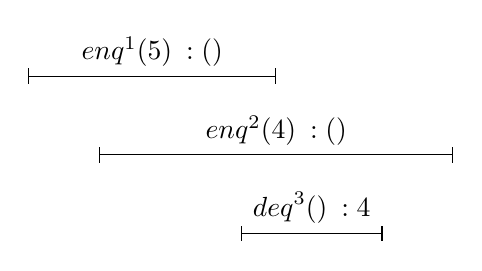
\begin{tikzpicture}[xscale = 0.9]
\draw[|-|] (0,0) -- node[above] {$\sm{enq}^1(5)\::()$} (3.5,0);
\draw (2.5,0) \X;
\draw[|-|] (1,-1) -- node[above] {$\sm{enq}^2(4)\::()$} (6,-1);
\draw (2,-1) \X;
\draw[|-|] (3,-2) -- node[above] {$\sm{deq}^3()\::4$} (5,-2);
\draw (4,-2) \X;
\end{tikzpicture}
\end{center}
\caption{Timeline representing the linearisation example.  Time runs from left
  to right; each horizontal line represents an operation execution, with the
  left-hand end representing the $\call$ event, and the right-hand end
  representing the $\return$ event.}
\label{fig:lin-timeline}
\scalaMid
\end{figure}

%%%%%

Linearisation is specified with respect to a linearisation specification
object~$Spec$, with the same operations (and signatures) as the concurrent
datatype in question.  A history of the specification object is a sequence of
events of the form:
%
\begin{itemize}
\item $op^i(x)\::y$ representing an execution of operation~$op$ with
  parameter~$x$, returning result~$y$; again $i$~is an execution identity,
  which must appear at most once in the history.
\end{itemize}
%
A history is \emph{legal} if it is consistent with the definition of~$Spec$,
i.e.~for each operation execution, the precondition is satisfied, and the
return value is as for the definition of the operation in~$Spec$.  In general,
the specification object could be nondeterministic, and so allow several
values that could be returned by an operation execution (although in all our
examples it will be deterministic).

%% We assume that the
%% specification object is deterministic: after a particular history, there is a
%% unique value that can be returned by each execution.

For example, consider the history
\begin{eqnarray*}
h_s & = & \seq{\sm{enq}^2(4)\::(),\; \sm{enq}^1(5)\::(),\; \sm{deq}^3()\::4}.
\end{eqnarray*}
%
This is a legal history for a specification object that represents a queue.
This history is illustrated by the ``$\cross$''s in
Figure~\ref{fig:lin-timeline}.

Let $h$ be a complete concurrent history, and let $h_s$ be a legal history of
the specification object~$Spec$.  We say that $h$ and~$h_s$ \emph{correspond}
if they contain the same executions, i.e., for each $\call.op^i(x)$ and
$\return.op^i\::y$ in $h$,\, $h_s$ contains $op^i(x)\::y$, and vice versa.  We
say that $h_s$ is a \emph{linearisation} of~$h$ if there is some way of
interleaving the two histories (i.e.~creating a history containing the events
of~$h$ and~$h_s$, preserving the order of events) such that each $op^i(x)\::y$
occurs between $\call.op^i(x)$ and $\return.op^i\::y$.  Informally, this
indicates that the executions of~$h$ appeared to take place in the order
described by~$h_s$, and that this order is legal according to the
specification object.  We say that $h$ is \emph{linearisable} with respect
to~$Spec$ in this case.

Continuing the running example, $h_s$ is a linearisation of~$h$, as evidenced
by the interleaving
\[
\seq{\begin{align}
  \call.\sm{enq}^1(5),\; \call.\sm{enq}^2(4),\; 
  \sm{enq}^2(4)\::(),\; \sm{enq}^1(5)\::(),\;   \call.\sm{deq}^3(), \\
  \return.\sm{enq}^1\::(),\; \sm{deq}^3\::4,\; 
  \return.\sm{deq}^3\::4,\; \return.\sm{enq}^2\::() },
  \end{align}
\]
as illustrated in  Figure~\ref{fig:lin-timeline}.
The points at which the events of~$h_s$ are inserted into~$h$ can be thought
of as the points where each operation has an effect; we refer to these as
\emph{linearisation points}. 

A concurrent history might not be complete, i.e.~it might have some pending
executions that have been called but have not returned.  An \emph{extension}
of a history~$h$ is formed by adding zero or more $\return$ events
corresponding to pending executions.  We write $complete(h)$ for the
subsequence of~$h$ formed by removing all $\call$ events corresponding to
pending executions.

We say that a (not necessarily complete) concurrent history~$h$ is
\emph{linearisable} with respect to specification object~$Spec$ if there is an
extension~$h'$ of~$h$ such that $complete(h')$ is linearisable with respect
to~$Spec$.  Informally, the $\return$ events that are in~$h'$ but not~$h$ are
for operation executions that have had an effect, but not returned in~$h$; the
$\call$ events removed in $complete(h')$ are for operation executions that
have not yet had an effect.

We say that a concurrent datatype is linearisable with respect to~$Spec$ if
each of its histories is linearisable with respect to~$Spec$.

%%%%%%%%%%%%%%%%%%%%%%%%%%%%%%%%%%%%%%%%%%%%%%%%%%%%%%%%%%%%

\subsection{Synchronisation linearisation}
\label{sec:sync-lin}

We now adapt the definition of linearisation to synchronisations.  With
standard linearisation, operations appear to take place in a one-at-a-time
order, each between the time at which the operation is invoked and when it
returns.  With synchronisation linearisation, synchronisations appear to take
place in a one-at-a-time order, with each synchronisation between the time
that each of the operations is invoked and when it returns.  In each case,
the order is one that satisfies the requirements captured by the specification
object.  

For the moment, we consider only binary heterogeneous synchronisations; we
generalise in the next section.  We consider a synchronisation object~$Sync$
with two operations, $\op_1$ and~$\op_2$, as described earlier.  A concurrent
history of~$Sync$ contains $\call$ and $\return$ events, as in the previous
subsection, corresponding to the operations~$\op_1$ and~$\op_2$.

For example, the following is a complete history of the synchronous channel
from earlier, and is illustrated in Figure~\ref{fig:sync-timeline}:
\begin{eqnarray*}
h & = & 
\seq{\begin{align}
  \call.\sm{send}^1(8),\; \call.\sm{send}^2(8),\; \call.\sm{receive}^3(()),\;
  \return.\sm{receive}^3\::8,\; \\
  \call.\sm{receive}^4(()),\; \return.\sm{send}^1\::(),\;
  \call.\sm{send}^5(9),\; \return.\sm{receive}^4\::9,\; \\
  \call.\sm{receive}^6(()),\; \return.\sm{send}^2\::(), \;
  \return.\sm{send}^5\::(),\; \return.\sm{receive}^6\::8 } .
  \end{align}
\end{eqnarray*}

%%%%%

\begin{figure}
\unScalaMid
\begin{center}
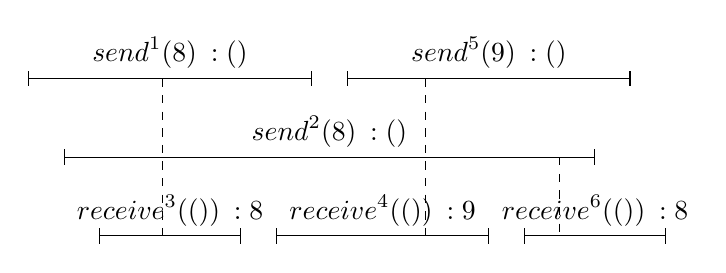
\begin{tikzpicture}[xscale = 0.9]
\draw[|-|] (0,0) -- node[above] {$\sm{send}^1(8)\::()$} (4,0);
\draw[|-|] (4.5,0) -- node[above] {$\sm{send}^5(9)\::()$} (8.5,0);
\draw[|-|] (0.5,-1) -- node[above] {$\sm{send}^2(8)\::()$} (8,-1);
\draw[|-|] (1,-2) -- node[above] {$\sm{receive}^3(())\::8$} (3,-2);
\draw[|-|] (3.5,-2) -- node[above] {$\sm{receive}^4(())\::9$} (6.5,-2);
\draw[|-|] (7,-2) -- node[above] {$\sm{receive}^6(())\::8$} (9,-2);
\draw (1.9,0) \X; \draw (1.9,-2) \X; 
\draw[dashed] (1.9,0) -- (1.9,-2); % sync 1 and 3
\draw (5.6,0) \X; \draw (5.6,-2) \X; 
\draw[dashed] (5.6,0) -- (5.6,-2); % sync 4 and 5
\draw (7.5,-1) \X; \draw (7.5,-2) \X; 
\draw[dashed] (7.5,-1) -- (7.5,-2); % sync 2 and 6 
\end{tikzpicture}
\end{center}
\caption{Timeline representing the synchronisation example.}
\label{fig:sync-timeline}
\scalaMid
\end{figure}


A history of a synchronisation specification object $Spec$ is a sequence of
events of the form $\sync^{i_1, i_2}(x_1, x_2)\:: (y_1, y_2)$, representing an
execution of |sync| with parameters $(x_1, x_2)$ and result $(y_1,y_2)$.  The
event's  identity is~$(i_1,i_2)$: each of~$i_1$ and~$i_2$ must
appear at most once in the history.  Informally, an event $\sync^{i_1,
  i_2}(x_1, x_2)\:: (y_1, y_2)$ corresponds to a synchronisation between
executions $\op_1^{i_1}(x_1)\::y_1$ and $\op_2^{i_2}(x_2)\::y_2$ in a history
of the corresponding synchronisation object.

A history is \emph{legal} if is consistent with the definition of the
specification object.
%
For example, the following is a legal history of |SyncChanSpec|.
\begin{eqnarray*}
h_s & = & 
\seq{
 \sm{sync}^{1,3}(8,()) \:: ((), 8), \;
 \sm{sync}^{5,4}(9,()) \:: ((), 9), \;
 \sm{sync}^{2,6}(8,()) \:: ((), 8) } .
\end{eqnarray*}
The history is illustrated by the ``$\cross$''s in
Figure~\ref{fig:sync-timeline}: each event corresponds to the synchronisation
of two operations, so is depicted by two ``$\cross$''s on the corresponding
operations, linked by a dashed vertical line.  
%
This particular synchronisation specification object is stateless, so in fact
any permutation of the history~$h_s$ would also be legal (but not all such
permutations will be compatible with the history of the synchronisation
object); but the same will not be true in general of a specification object
with state.
%
The points at which the events of~$h_s$ are inserted into~$h$ can be thought
of as the points where each synchronisation takes place; we refer to these as
\emph{synchronisation points}. 

%
\begin{definition}
Let $h$ be a complete history of the synchronisation object~$Sync$.  We say
that a legal history~$h_s$ of~$Spec$ \emph{corresponds} to~$h$ if their
events agree; more precisely:
\begin{itemize}
\item For each  $\sync^{i_1, i_2}(x_1, x_2)\:: (y_1, y_2)$ in~$h_s$,\,
  $h$ contains events $\call.\op_1^{i_1}(x_1)$,\,
  $\return.\op_1^{i_1}\::y_1$\,, $\call.\op_2^{i_2}(x_2)$, and
  $\return.\op_2^{i_2}\::y_2$.

\item For each $\call.\op_1^{i_1}(x_1)$ and $\return.\op_1^{i_1}\::y_1$
  in~$h$,\, $h_s$ contains an event $\sync^{i_1, i_2}(x_1, x_2)\:: (y_1, y_2)$
  for some~$i_2$, $x_2$, and~$y_2$.

\item For each $\call.\op_2^{i_2}(x_2)$ and $\return.\op_2^{i_2}\::y_2$
  in~$h$,\, $h_s$ contains an event $\sync^{i_1, i_2}(x_1, x_2)\:: (y_1, y_2)$
  for some~$i_1$, $x_1$, and~$y_1$.
\end{itemize}
%% %
%% \begin{itemize}
%% \item For each |sync| event with identity~$(i_1,i_2)$ in~$h_s$,\, $h$ contains
%%   an execution of~$\op_1$ with identity~$i_1$ and an execution of~$\op_2$ with
%%   identity~$i_2$;

%% \item For each execution of~$\op_1$ with identity~$i_1$ in~$h$,\, $h_s$
%%   contains a |sync| event with identity~$(i_1,i_2)$ for some~$i_2$;

%% \item For each execution of~$\op_2$ with identity~$i_2$ in~$h$,\, $h_s$
%%   contains a |sync| event with identity~$(i_1,i_2)$ for some~$i_1$.
%% \end{itemize}
\end{definition}

\begin{definition}
Given a complete history $h$ of~$Sync$ and a corresponding legal history $h_s$
of~$Spec$, we say that $h_s$ is a \emph{synchronisation linearisation} of~$h$
if there is some way of interleaving $h$ and~$h_s$ such that each event
$\sync^{i_1, i_2}(x_1, x_2)\:: (y_1, y_2)$ occurs between
$\call.\op_1^{i_1}(x_1)$ and $\return.\op_1^{i_1}\::y_1$, and between
$\call.\op_2^{i_2}(x_2)$ and $\return.\op_2^{i_2}\::y_2$.
\end{definition}
%
%% We say that $h$ is \emph{synchronisation-linearisable} with respect to~$Spec$
%% in this case.  
In~the running example, $h_s$ is a synchronisation
linearisation of~$h$, as shown by the interleaving in
Figure~\ref{fig:sync-timeline}.

\begin{definition}
\label{def:sync-lin-objects}
Given a (not necessarily complete) concurrent history~$h$ and a corresponding
legal history~$h_s$ of $Spec$, we say that $h_s$ is a \emph{synchronisation
  linearisation} of~$h$ if there is an extension~$h'$ of~$h$ such that $h_s$
is a synchronisation linearisation of $complete(h')$.
%
We say that $h$ is synchronisation-linearisable with respect to~$Spec$ in this
case.  We say that a synchronisation object is synchronisation-linearisable
with respect to~$Spec$ if each of its histories is
synchronisation-linearisable with respect to~$Spec$.
\end{definition}

Informally, the $\return$ events that are
in~$h'$ but not~$h$ are for operation executions that have synchronised, but
not returned in~$h$; the $\call$ events removed in $complete(h')$ are for
operation executions that have not yet synchronised.


 % formal definition of synchronisation linearisation
\subsection{Variations}
\label{ssec:spec-variations}

Above we considered heterogeneous binary synchronisations,
i.e.~synchronisations between \emph{two} executions of \emph{different}
operations, with a single mode of synchronisation.  In this section, we
generalise.  There are two aspects of this: defining the effect of a
synchronisation, via a synchronisation specification object; and defining
which operations of the synchronisation object can synchronise together, and
relating them to the corresponding operation of the synchronisation
specification object.

It is straightforward to generalise to synchronisations between an arbitrary
number of operation executions, some of which might be executions of the same
operation.  Consider a $k$-way synchronisation between operations
\begin{scala}
def op£\s j£(x£\s j£: A£\s j£): B£\s j£   £for $j = 1, \ldots, k,$£
\end{scala}
%
where the $\op_j$ might not be distinct.
The specification object will have a corresponding operation of the form
%
\begin{scala} 
def sync(x£\s1£: A£\s1£, ..., x£\s k£: A£\s k£): (B£\s1£, ..., B£\s k£)
\end{scala}
%
For example, for the combining barrier |CombiningBarrier(n, f)| of the
Introduction, the corresponding specification object would be\footnote{We
  change the name of the operation to~{\scalashape syncA}, to avoid a
  name-clash with the operation {\scalashape sync} of {\scalashape
    CombiningBarrier}.}   
% [A](n: Int, f: (A,A) => A)
\begin{scala}
class CombiningBarrierSpec{
  def syncA((id£\s1£,x£\s1£): (Int,A) ..., (id£\s{\ss n}£,x£\s{\ss n}£): (Int,A)) = {
    val result = f(x£\s1£, f(x£\s2£,...f(x£\s{{\ss{n}}-1}£, x£\s{\ss n}£)...)); (result,...,result)
  }
}
\end{scala}

We define the relationship between operations of the synchronisation object
and of the synchronisation specification object via a \emph{synchronisation
  abstraction function}: this is a partial function that maps a (non-empty)
sequence of operations of the synchronisation object to the corresponding
operation of the synchronisation specification object.  For the combining
barrier, the abstraction function is
\[
\begin{align}
\set{ 
  \seq{ \sm{sync}((id_1,x_1)), \ldots, \sm{sync}((id_{\ss n},x_{\ss n})) } \mapsto
  \sm{syncA}((id_1,x_1), \ldots, (id_{\ss n},x_{\ss n})) 
 \midd \\
\qquad id_1, \ldots id_{\ss n} \in \sm{Int}, x_1,\ldots,x_{\ss n} \in \sm A
}.
\end{align}
\]
%% (The former |sync|s represent the operation in |CombiningBarrier|,
%% and the latter |sync| represents the operation of the same name in
%% |Combining|\-|Barrier|\-|Spec|.) 

For the generic binary synchronisations we considered in
Section~\ref{sec:sync-lin}, the abstraction function is
\[
\set{ \seq{\op_1(x_1), \op_2(x_2)} \mapsto \sync(x_1,x_2) \midd 
  x_1 \in \sm A_1, x_2 \in \sm A_2 }.
\]

For a synchronisation object with multiple modes of synchronisation, the
synchronisation specification object has a different operation for each mode.
For example, recall the |TimeoutChannel| from the Introduction, where sends
and receives may timeout and return without synchronisation.  The
corresponding specification object is as follows (we omit arguments of
type~|Unit|, to improve readability).
%
\begin{scala}
class TimeoutChannelSpec[A]{
  def sendTO(x: A) = false       // £send£ times out.
  def receiveTO() = None  // £receive£ times out.
  def sync(x: A) = (true, Some(x))  // Synchronisation.
}
\end{scala}
%
The operation |sendTO| corresponds to a send timing out (and so not
synchronising), |receiveTO| corresponds to a receive timing out, and
|sync| corresponds to a send and receive synchronising.  This is
formalised by the synchronisation abstraction function:
\[
\begin{align}
\set{ \seq{ \sm{send}(x) } \mapsto \sm{sendTO}(x)  \midd x \in \sm A } \union{} 
\set{ \seq{ \sm{receive}() } \mapsto \sm{receiveTO}()  } \union{}  \\
\set{ ( \seq{ \sm{send}(x), \sm{receive}() } \mapsto \sm{sync}(x) \midd
      x \in \sm A }.
\end{align}
\]

As another example, the following is a specification object for a channel with
a close operation.
%
%\begin{mysamepage}
\begin{scala}
class ClosableChannelSpec[A]{
  private var isClosed = false  // Is the channel closed? 
  def close() = { isClosed = true; () }
  def sync(x: A) = { require(!isClosed); ((), x) }
  def sendFail(x: A) = { require(isClosed); throw new Closed }
  def receiveFail() = { require(isClosed); throw new Closed }
}
\end{scala}
%\end{mysamepage}
%
The synchronisation abstraction function is
\[
\begin{align}
\set{ \seq{\sm{close}()} \mapsto \sm{close}() }  \union 
\set{ \seq{ \sm{send}(x), \sm{receive}() } \mapsto \sm{sync}(x) \midd
      x \in \sm A } \union\null \\
\set{ \seq{ \sm{send}(x) } \mapsto \sm{sendFail}(x)  
  \midd x \in \sm A } \union{} 
\set{ \seq{ \sm{receive}() } \mapsto \sm{receiveFail}()  }.
\end{align}
\]
A send and receive can synchronise corresponding to |sync|, but only before
the channel is closed; or each may fail once the channel is closed,
corresponding to |sendFail| and |receiveFail|.  

We now describe how to generalise the definition of synchronisation
linearisation.  Fix a synchronisation specification object $Spec$ and
corresponding synchronisation abstraction function~$\A$.  For each operation
\begin{scala}
  def £$sync$£(x£\s 1£: A£\s 1£,...,x£\s n£: A£\s k£): (B£\s 1£,...,B£\s k£) 
\end{scala}
of $Spec$ (corresponding to $k$ threads synchronising), we introduce events
$sync^{i_1, \ldots, i_k}(x_1, \ldots, x_k)\:: (y_1, \ldots, y_k)$ (where,
for each~$j$,\, $x_j \in A_j$,\, $y_j \in B_j$, and $i_j$ is an execution
identity).  A legal history of $Spec$ is then a sequence of such events,
consistent with the definition of $Spec$.

\begin{definition}
\label{def:sync-lin}
Let $h$ be a complete history of the synchronisation object.  Then a legal
history $h_s$ of~$Spec$ corresponds to $h$ if:
\begin{itemize}
\item
For each event $sync^{i_1, \ldots, i_k}(x_1, \ldots, x_k)\:: (y_1, \ldots,
y_k)$ in~$h_s$, there is some maplet $\seq{ op_1(x_1), \ldots, op_k(x_k) } \mapsto
sync(x_1,\ldots,x_k)$ in~$\A$ such that, for
each~$j$, $h$ contains an execution of $op_j(x_j)^{i_j}\:: y_j$.

\item For each execution $op_j(x_j)^{i_j}\:: y_j$ in~$h$,\, $h_s$ contains
  some event of the form $sync^{i_1, \ldots, i_k}(x_1, \ldots, x_k)\:: (y_1,
  \ldots, y_k)$ (necessarily the abstraction function~$\A$ relates operations
  as in the previous bullet point).
\end{itemize}
%
Then $h_s$ is a synchronisation linearisation of~$h$ if there is some way of
interleaving $h$ and~$h_s$ such that each event $sync^{i_1, \ldots, i_k}(x_1,
\ldots, x_k)\:: (y_1, \ldots, y_k)$ is between $\call.op_j^{i_j}(x_j)$
and $\return.op_j^{i_j}\::y_j$, for each~$j$. 
\end{definition}

The definition of synchronisation-linearisability follows in the obvious
way.

%% %
%% The definition of synchronisation linearisation is an obvious adaptation of
%% the earlier definition: in the interleaving of the complete history of the
%% synchronisation history and the history of the specification object, each
%% $\sm{sync}^{i_1, \ldots, i_k}(x_1, \ldots, x_k)\:: (y_1, \ldots, y_k)$ occurs
%% between $\call.\op_1^{i_j}(x_j)$ and $\return.\op_j^{i_j}\::y_j$ for each $j =
%% 1, \ldots, k$.
%% %% The definition of synchronisation-linearisability follows in the obvious
%% %% way.

%% Note that if several of the $\op_j$ are the same operation, there is a choice
%% as to the order in which their parameters are passed to |sync|.  (However, in
%% the case of the combining barrier, if |f| is associative and commutative, the
%% order makes no difference.)

%% It is also straightforward to adapt the definitions to deal with multiple
%% modes of synchronisation: the specification object has a different operation
%% for each mode.  For example, recall the |TimeoutChannel| from the
%% Introduction, where sends and receives may timeout and return without
%% synchronisation.  The corresponding specification object would be:
%% %
%% \begin{scala}
%% class TimeoutChannelSpec[A]{
%%   def sync£\s s£(x: A) = false       // £send£ times out.
%%   def sync£\s r£(u: Unit) = None  // £receive£ times out.
%%   def sync£\s{s,r}£(x: A, u: Unit) = (true, Some(x))  // Synchronisation.
%% }
%% \end{scala}
%% %
%% The operation $\sm{sync}_s$ corresponds to a send returning without
%% synchronising; likewise $\sm{sync}_r$ corresponds to a receive returning
%% without synchronising; and $\sm{sync}_{s,r}$ corresponds to a send and receive
%% synchronising.  The formal definition of synchronisation linearisation is the
%% obvious adaptation of the earlier definition: in particular |sync|\s{s} must
%% occur between the call and return of a send that doesn't synchronise, and
%% likewise for |sync|\s{r}.

%% As another example, the following is a specification object for a channel with
%% a close operation.
%% %
%% \begin{mysamepage}
%% \begin{scala}
%% class ClosableChannelSpec[A]{
%%   private var isClosed = false  // Is the channel closed? 
%%   def close(u: Unit) = { isClosed = true; () }
%%   def sync(x: A, u: Unit) = { require(!isClosed); ((), x) }
%%   def sendFail(x: A) = { require(isClosed); throw new Closed }
%%   def receiveFail(u: Unit) = { require(isClosed); throw new Closed }
%% }
%% \end{scala}
%% \end{mysamepage}
%% %
%% A send and receive can synchronise corresponding to |sync|, but only before
%% the channel is closed; or each may fail once the channel is closed,
%% corresponding to |sendFail| and |receiveFail|. 

%%%%%%%%%%%%%%%%%%%%%%%%%%%%%%%%%%%%%%%%%%%%%%%%%%%%%%%

\subsection{Locality}
\label{sec:locality}

So far, we have implicitly assumed a single synchronisation object.  However,
a program may employ multiple synchronisation objects.  Consider a set of
independent synchronisation objects~$\O$.  Given a history~$h$ and an
object~$o$, we write $h \restrict o$ for the restriction of $h$ to events
of~$o$.  We assume that the objects are independent, so $h$ is a history
of~$\O$ if and only if $h \restrict o$ is a history of~$o$ for each~$o$. 

We assume that each synchronisation object~$o$ has its own synchronisation
specification object $Spec_o$ and abstraction function~$\A_o$.  We can combine
the specification objects into a single specification object~$Spec$, with the
operations of all $Spec_o$ (assumed distinct): a history~$h_s$ is legal if and
only if $h_s \restrict Spec_o$ is legal for each $Spec_o$.  Likewise we can
combine the abstraction functions into a single abstraction function~$\A$, by
taking their union.

We show that synchronisation linearisation satisfies a locality property: the
objects~$\O$ are synchronisation-linearisable if and only if each individual
object is synchronisation-linearisable.  This is an important result, as it
allows for compositional development and verification.  

\begin{lemma}
\label{lem:local}
Let $h$ be a complete history of the synchronisation objects~$\O$.
Then $h$ is synchronisation-linearisable (with respect to $Spec$ and~$\A$) if
and only if $h \restrict o$ is synchronisation-linearisable (with respect to
$Spec_o$ and $\A_o$), for each~$o \in \O$.
%% , and $h_s$ a legal history~$h_s$ of~$Spec$.  Then $h_s$ is a
%% synchronisation linearisation of~$h$ if and only if $h_s \restrict Spec_o$
%% is a synchronisation linearisable of $h \restrict o$, for each~$o$.
\end{lemma}

\begin{proof}
The left-to-right implication is trivial.  

For the right-to-left implication, suppose that $h \restrict o$ is
synchronisation-linearisable, for each~$o$.  That means that there is a legal
history~$h_{s_o}$ of~$Spec_o$ that is a synchronisation linearisation of~$h
\restrict o$.  Write $h^I_o$ for the interleaving of these histories that
demonstrates this (following Definition~\ref{def:sync-lin}).

We build an interleaving~$h^I$ of~$h$ and all $h_{s_o}$ for $o \in \O$,
consistent with the $h^I_o$ interleavings: if, in~$h^I_o$, a $\call$ or
$\return$ event~$e$ of~$o$ is followed by events $s_1,\ldots,s_k$ of
$h_{s_o}$, then we insert $s_1,\ldots,s_k$ into~$h$ directly after~$e$.

In the resulting interleaving~$h^I$, each synchronisation event is still
between the relevant $\call$ and $\return$ events, by construction.  Let $h_s$
be the restriction of~$h^I$ to the events of the specification
objects.  Then for each~$o$,\, $h_s \restrict Spec_o = h_{s_o}$, by
construction, so is legal.  Hence $h_s$ is legal.
\end{proof}

\begin{prop}
The collection of objects~$\O$ is synchronisation-linearisable (with respect
to $Spec$ and~$\A$) if and only if $o$ is synchronisation-linearisable (with
respect to~$Spec_o$ and $\A_o$), for each $o \in \O$.
\end{prop}
%
\begin{proof}
The left-to-right implication is again trivial.  

For the right-to-left implication, consider a (not necessarily complete)
history~$h$ of~$\O$.  For each $o$, since $o$ is synchronisation-linearisable,
there is an extension $h_o'$ of $h \restrict o$ such that $complete(h_o')$ is
synchronisation-linearisable with respect to $Spec_o$ and~$\A_o$.
%
Let $h'$ be an extension of~$h$, adding the events in each~$h_o'$ but
not~$h_o$ in the same order (but interleaving events from different of
different objects arbitrarily).  Then $complete(h') \restrict o =
complete(h_o')$, for each~$o$.
%
Then $complete(h')$ is a complete history of~$\O$, and by
Lemma~\ref{lem:local}, $complete(h')$ is synchronisation-linearisable with
respect to~$Spec$ and~$\A$, as required.
\end{proof}

 % variations, progress.
\section{Relating synchronisation and linearisation}

In this section we describe the relationship between synchronisation
linearisation and standard linearisation.  

\framebox{\ldots}

It is clear that synchronisation linearisation cannot, in general, be captured
directly as standard linearisation.  More precisely, given a synchronisation
linearisability specification object $SyncSpec$, it is not, in general,
possible to find a linearisability syncronisation specification $Spec$ such
that for every history~$h$,\, $h$ is synchronisation linearisable with respect
to $SyncSpec$ if and only if $h$ is linearisable with respect to $Spec$.

For example, consider the example of a synchronous channel from
Section~\ref{sec:spec}, where synchronisation linearisation is captured by
|SyncChanSpec|.  Assume (for a contradiction) that the same property can be
captured by linerisation with respect to linearisability specification~$Spec$.
Consider the history
\begin{eqnarray*}
h & = & \seq{ 
  \call.send^1(3), \call.receive^2(), 
  \return.send^1\::(), \return.receive^2()\::3 }.
\end{eqnarray*}
%
This is synchronisation linearisable with respect to |SyncChanSpec|.  By the
assumption, there must be a legal history~$h_s$ of~$Spec$ such that $h$
and~$h_s$ are compatible.  Without loss of generality, suppose the |send|
in~$h_s$ occurs before the~|receive|, i.e.
\begin{eqnarray*}
h_s & = & \seq{ send^1(3)\::(), receive^2()\::3 }.
\end{eqnarray*}
%
But the history
%
\begin{eqnarray*}
h' & = & \seq{ 
  \call.send^1(3), \return.send^1\::(), 
  \call.receive^2(), \return.receive^2()\::3 }
\end{eqnarray*}
%
is also compatible with respect to~$h_s$, so $h'$ is linearisable with respect
to~$Spec$.  But then the assumption would imply that $h'$ is synchronisation
linearisable with respect to~|SyncChanSpec|.  This is clearly false, because
the operations do not overlap.  Hence no such  linearisability
specification~$Spec$ exists.


%%%%%%%%%%%%%%%%%%%%%%%%%%%%%%%%%%%%%%%%%%%%%%%%%%%%%%%

\subsection{Two-step linearisability}

In the previous section, we showed that synchronisation linearisation does not
correspond directly to linearisation.  Nevertheless, we will show that
synchronisation linearisability corresponds to a small adaptation of
linearisability, but where one of the operations on the concurrent object
corresponds to \emph{two} operations of the linearisability specification
object.  We define what we mean by this, and then prove the correspondence in
the next subsection.  In the definitions below, we describe just the
differences from standard linearisation, to avoid repetition.

Given a synchronisation object with operations |op|\s1 and |op|\s2, as before,
we will consider a linearisability specification object with signature
%
\begin{scala}
object TwoStepLinSpec{
  def op£\s1£(x£\s1£: A£\s1£): Unit
  def £$\overline{\sm{op}}_1$£(): B£\s1£
  def op£\s2£(x£\s2£: A£\s2£): B£\s2£
}
\end{scala}
%
The idea is that the operation |op|\s1 on the concurrent object will be
linearised by the composition of the two operations |op|\s1 and
$\overline{\sm{op}}_1$; but operation |op|\s2 on the concurrent object will be
linearised by just the operation |op|\s2 of the specification object, as
before.  We call such an object a \emph{two-step linearisability specification
  object}. 

We define a history~$h_s$ of such a two-step specification object much as in
Section~\ref{sec:specification-linearisability}, except that for each event
$\overline{\sm{op}}_1^i()\::y$ in~$h_s$, we require that there is an
earlier event |op|$_1^i(x)\::()$ in~$h_s$ with the same invocation
identity; other than in this regard, invocation identities are not repeated
in~$h_s$.

Let $h$ be a complete concurrent history of a synchronisation object, and let
$h_s$ be a legal history of a two-step specification object corresponding to
the same invocations in the following sense:
%
\begin{itemize}
\item For every $\call.\sm{op}_1^i(x)$ and $\return.\sm{op}_1^i\::y$ in $h$,\,
  $h_s$~contains $\sm{op}_1^i(x)\::()$ and $\overline{\sm{op}}_1^i()\::y$; and
  vice versa;

\item For every $\call.\sm{op}_2^i(x)$ and $\return.\sm{op}_2^i\::y$ in $h$,\,
  $h_s$~contains $\sm{op}_2^i(x)\::y$; and vice versa.
\end{itemize}
%
We say that $h$ and $h_s$ are \emph{two-step compatible} if there is some way of
interleaving the two histories such that 
%
\begin{itemize}
\item Each $\sm{op}_1^i(x)\::()$ and $\overline{\sm{op}}_1^i()\::y$ occur
  between $\call.\sm{op}_1^i(x)$ and $\return.\sm{op}_1^i\::y$, in that
  order; 

\item Each $\sm{op}_2^i(x)\::y$ occurs between $\call.\sm{op}_2^i(x)$ and
  $\return.\sm{op}_2^i\::y$.
\end{itemize}

For example, consider a synchronous channel, with |send| corresponding
to~$op_1$, and |receive| corresponding to~$op_2$.  Then the following would be
an interleaving of two-step compatible histories of the synchronisation object
and the corresponding specification object.
\[
\seq{\begin{align} 
 \call.\sm{send}^1(3),\; \sm{send}^1(3)\::(),\; 
 \call.\sm{receive}^2(),\; \sm{receive}^2()\::3,\; \\
 \overline{\sm{send}}^1()\::(),\; \return.\sm{send}^1\::(), \;
 \return.\sm{receive}^2\::3 }.
\end{align}
\]

The definition of two-step linearisability then follows from this definition
of two-step compatability, precisely as in
Section~\ref{sec:specification-linearisability}.



%%%%%%%%%%%%%%%%%%%%%%%%%%%%%%%%%%%%%%%%%%%%%%%%%%%%%%%

\subsection{Proving the relationship}
\label{sec:twoStepLinSpec}

We now prove the relationship between synchronisation linearisation and
two-step linearisation.

Consider a synchonisation specification object |SyncSpec|.  We build a
corresponding two-step linearisation specification object~|TwoStepLinSpec|
such that synchronisation linearisation with respect to |SyncSpec| is
equivalent to two-step linearisation with respect to~|TwoStepLinSpec|.  The
definition is below: the specification's behaviour is described by the
automaton on the right.\footnote{Defining the subclasses of {\scalashape
    State} as {\scalashape case class}es allows pattern matching against such
  values.  For example, the statement {\scalashape val One(x}\s1{\scalashape )
    = state} succeeds only if {\scalashape state} has type {\scalashape One},
  and binds the name {\scalashape x}\s1 to the value of the {\scalashape x}\s1
  field of {\scalashape state}.}
\begin{trivlist}
\item[]
\begin{minipage}[b]{68mm}
\begin{scala}
trait State
case class Zero extends State
case class One(x£\s1£: A£\s1£) extends State
case class Two(y£\s1£: B£\s1£) extends State
\end{scala}
\end{minipage}
%
\hfil
%
\begin{minipage}[b]{63mm}
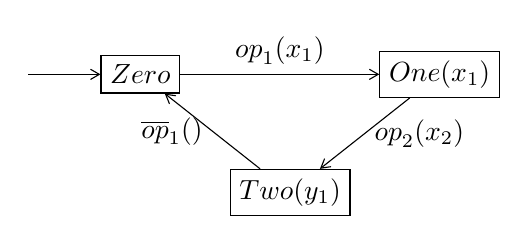
\begin{tikzpicture}[>= angle 60, xscale = 0.95, yscale = 0.75]
\draw (0,0) node[draw] (zero) {$\sm{Zero}$};
\draw[->] (zero) ++ (-1.5, 0) -- (zero);
%
\draw (4,0) node[draw] (one) {$\sm{One}(\sm{x}_1)$};
\draw[->] (zero)  -- node[above] {$\sm{op}_1(\sm{x}_1)$} (one); 
%
\draw (2, -2) node[draw] (two) {$\sm{Two}(\sm{y}_1)$};
\draw[->] (one)  -- node[right] {$\sm{op}_2(\sm{x}_2)$} (two); 
\draw[->] (two) -- node[left] {$\overline{\sm{op}}_1()$} (zero);
\end{tikzpicture}
\end{minipage}
%
%The specification object is defined as follows.
%
%% trait LinState
%% case class Zero extends LinState
%% case class One(x£\s1£: A£\s1£) extends LinState
%% case class Two(y£\s1£: B£\s1£) extends LinState
%
\begin{scala}
object TwoStepLinSpec{
  private var state: State = Zero
  def op£\s1£(x£\s1£: A£\s1£): Unit = {
    require(state.isInstanceOf[Zero]); state = One(x£\s1£)
  }
  def op£\s2£(x£\s2£: A£\s2£): B£\s2£ = {
    require(state.isInstanceOf[One]); val One(x£\s1£) = state
    val (y£\s1£, y£\s2£) = SyncSpec.sync(x£\s1£, x£\s2£); state = Two(y£\s1£); y£\s2£
  }
  def £$\overline{\sm{op}}_1$£(): B£\s1£ = {
    require(state.isInstanceOf[Two]); val Two(y£\s1£) = state; state = Zero; y£\s1£
  }
}
\end{scala}
\end{trivlist}
%
%
The definition forces the operations to take place in the order described by
the automaton.  In addition, the |op|\s2 operation calls the |sync| method on
|SyncSpec|, to calculate the return values and to update |SyncSpec|'s state;
it stores |op|\s1's result in the state. 

% in effect, the synchronisation happens at this point.

The following lemma follows immediately from the construction
of~|Two|\-|Step|\-|LinSpec|. 
%
\begin{lemma}
\label{lem:TwoStepLinSpec-histories}
Each history of~|TwoStepLinSpec| is the concatenation of triples of events of
the form $\sm{op}_1^{i_1}(x_1) \:: ()$,\, $\sm{op}_2^{i_2}(x_2) \:: y_2$,\,
$\overline{\sm{op}}_1^{i_1}() \:: y_1$ such that |SyncSpec| has a
corresponding legal history of events $\sm{sync}^{i_1,i_2}(x_1,x_2) \::
(y_1,y_2)$, and vice versa.
\end{lemma}

%%%%%

The following proposition reduces synchronisation linearisability to two-step
linearisability.
%
\begin{prop}
Let |SyncObj| be a synchronisation object, |SyncSpec| be a synchronisation
specification object, and let |TwoStepLinSpec| be built from |SyncSpec| as
above.  Then |SyncObj| is two-step linearisable with respect to
|Two|\-|Step|\-|LinSpec| if and only if it is synchronisation linearisable
with respect to |SyncSpec|.
\end{prop}
%%%%%%
\begin{proof}
\textbf{($\implies$).}\quad
%
Let $h$ be a concurrent history of |SyncObj|.  By assumption, there is an
extension $h'$ of~$h$, and a legal history~$h_s$ of |TwoStepLinSpec| such that
$h'' = complete(h')$ and~$h_s$ are two-step compatible.
%
Build a history~$h_s'$ of |SyncSpec| by replacing each triple
$\sm{op}_1^{i_1}(x_1) \:: ()$,\, $\sm{op}_2^{i_2}(x_2) \:: y_2$,\,
$\overline{\sm{op}}_1^{i_1}() \:: y_1$ in~$h_s$ by the event
$\sm{sync}^{i_1,i_2}(x_1,x_2) \:: (y_1,y_2)$.  
%
The history~$h_s'$ is legal by Lemma~\ref{lem:TwoStepLinSpec-histories}.  
%
It is possible to interleave $h''$ and~$h_s'$ by placing each event
$\sm{sync}^{i_1,i_2}(x_1,x_2) \:: (y_1,y_2)$ in the same place as the
corresponding event $\sm{op}_2^{i_2}(x_2) \:: y_2$ in the interleaving
of~$h''$ and~$h_s$; by construction, this is between
$\call.\sm{op}_1^{i_1}(x_1)$ and~$\return.\sm{op}_1^{i_1} \:: y_1$, and
between $\call.\sm{op}_2^{i_2}(x_2)$ and~$\return.\sm{op}_2^{i_2} \:: y_2$.
%
Hence $h''$ and~$h_s$ are synchronisation compatible, so $h''$ is
synchronisation lineariable, and so $h$ is synchronisation linearisable.

%%%%%

\textbf{($\Leftarrow$).}\quad
%
Let $h$ be a complete history of |SyncObj|.  By assumption, there is an
extension $h'$ of~$h$, and a legal history~$h_s$ of |SyncSpec| such that $h''
= complete(h')$ and~$h_s$ are synchronisation compatible.
%
Build a history~$h_s'$ of |TwoStepLinSpec| by replacing each event
$\sm{sync}^{i_1,i_2}(x_1,x_2) \:: (y_1,y_2)$ in~$h_s$ by the three events
$\sm{op}_1^{i_1}(x_1) \:: ()$,\, $\sm{op}_2^{i_2}(x_2) \:: y_2$,\,
$\overline{\sm{op}}_1^{i_1}() \:: y_1$.
%
The history~$h_s'$ is legal by Lemma~\ref{lem:TwoStepLinSpec-histories}.
%
It is possible to interleave $h''$ and~$h_s'$ by placing each triple
$\sm{op}_1^{i_1}(x_1) \:: ()$,\, $\sm{op}_2^{i_2}(x_2) \:: y_2$,\,
$\overline{\sm{op}}_1^{i_1}() \:: y_1$ in the same place as the corresponding
event $\sm{sync}^{i_1,i_2}(x_1,x_2) \:: (y_1,y_2)$ in the interleaving
of~$h''$ and~$h_s$; by construction, each $\sm{op}_1^{i_1}(x_1) \:: ()$ and
$\overline{\sm{op}}_1^{i_1}() \:: y_1$ are between
$\call.\sm{op}_1^{i_1}(x_1)$ and~$\return.\sm{op}_1^{i_1} \:: y_1$; and each
$\sm{op}_2^{i_2}(x_2) \:: y_2$ is between $\call.\sm{op}_2^{i_2}(x_2)$
and~$\return.\sm{op}_2^{i_2} \:: y_2$.
%
Hence $h''$ and~$h_s$ are two-step compatible, so $h''$ is two-step
lineariable, and so $h$ is two-step linearisable.
\end{proof}

%%%%%%%%%%

The two-step linearisation specification object can often be significantly
simplified from the template definition above.  Here is such a specification
object for a synchronous channel.
%
\begin{scala}
object SyncChanTwoStepLinSpec{
  private var state = 0        // Takes values 0, 1, 2, cyclically 
  private var value: A = _    // The current value being sent
  def send(x: A): Unit = { require(state == 0); value = x; state = 1 }
  def receive(u: Unit): A = { require(state == 1); state = 2; value }
  def £$\overline{\sm{send}}$£(): Unit = { require(state == 2); state = 0 }
}
\end{scala}
 % relating synchronisation linearisation and linearisation
\subsection{Variations}
\label{ssec:relating-variations}

We now discuss some variations on the case of binary heterogeneous
synchronisations in the previous section.  We give a general construction in
the next section, but we consider the constructions in this section to be
easier to understand: to a certain extent, this section can be seen as
providing stepping stones towards that general construction. 

The results of the previous subsections carry across to non-binary, fixed
arity synchronisations, in a straightforward way.  For a $k$-way
synchronisation between distinct operations |op|\s1, \ldots, |op|$_k$, the
corresponding two-step linearisation specification object has $2k-1$
operations, |op|\s1, \ldots, |op|$_k$, $\overline{\sm{op}}_1$, \ldots,
$\overline{\sm{op}}_{k-1}$.  The definition of two-step linearisation is then
the obvious adaptation of the binary case: each operation |op|\s{i} of the
synchronisation object is linearised by the composition of |op|\s{i} and
$\overline{\op}_i$ of the specification object, for $i = 1, \ldots, k-1$.

The construction of the previous subsection is easily adapted to the case of
$k$-way synchronisations for $k > 2$.  The specification object encodes an
automaton with $k$ states.  The figure below gives the automaton in the case
$k = 4$.
%
\begin{center}
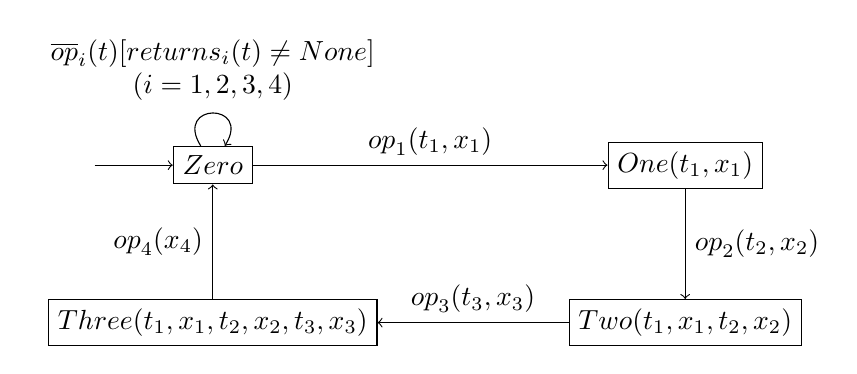
\begin{tikzpicture}[xscale = 1]
\draw (0,0) node[draw] (zero) {$\sm{Zero}$};
\draw[->] (zero) ++ (-1.5, 0) -- (zero);
\draw[->] (zero) .. controls ++(-0.5,+0.8) and ++(0.5,0.8) .. 
  node[above]{
    $\begin{array}{c}
      \overline{\op}_i(t) [\sm{returns}_i(t) \ne \sm{None}] \\ (i = 1,2,3,4)
    \end{array}$}
  (zero);
%
\draw (zero)++(6,0) node[draw] (one) {$\sm{One}(\sm{t}_1, \sm{x}_1)$};
\draw[->] (zero)  -- node[above] {$\sm{op}_1(\sm{t}_1, \sm{x}_1)$} (one); 
%
\draw (one)++(0, -2) node[draw] (two) 
  {$\sm{Two}(\sm{t}_1, \sm{x}_1, \sm{t}_2, \sm{x}_2)$};
\draw[->] (one)  -- node[right] {$\sm{op}_2(\sm{t}_2, \sm{x}_2)$} (two); 
%
\draw (two)++(-6, 0) node[draw] (three) 
  {$\sm{Three}(\sm{t}_1, \sm{x}_1, \sm{t}_2, \sm{x}_2, \sm{t}_3, \sm{x}_3)$};
\draw[->] (two)  -- node[above] {$\sm{op}_3(\sm{t}_3, \sm{x}_3)$} (three); 
%
\draw[->] (three)  -- node[left] {$\sm{op}_4(\sm{x}_4)$} (zero);
\end{tikzpicture}
\end{center}
%
The final |op| operation, |op|\s4 in the above figure, applies the |sync|
method of the synchronisation specification object to the parameters $\sm x_1,
\ldots, \sm x_k$ to obtain the results $\sm y_1, \ldots, \sm y_k$; it stores
the first $k-1$ in appropriate |returns|\s{i} arrays, and returns $\sm y_k$
itself.  In the case $k=4$, it has definition:
%
\begin{scala}
  def op£\s4£(x£\s4£: A£\s4£): B£\s4£ = {
    require(state.isInstanceOf[Three]); val Three(t£\s1£, x£\s1£, t£\s2£, x£\s2£, t£\s3£, x£\s3£) = state
    val (y£\s1£, y£\s2£, y£\s3£, y£\s4£) = SyncSpec.sync(x£\s1£, x£\s2£, x£\s3£, x£\s4£) 
    returns£\s1£(t£\s1£) = Some(y£\s1£); returns£\s2£(t£\s2£) = Some(y£\s2£); returns£\s3£(t£\s3£) = Some(y£\s3£)
    state = Zero; y£\s4£
  }
\end{scala}
%
Each $\overline{\sm{op}}_i$ operation retrieves the result from the
corresponding |returns|\s{i} array.

%%%%%%%%%%%%%%%%%%%%%%%%%%%%%%%%%%%%%%%%%%%%%%%%%% Homogeneous

\begin{window}[0,r,{%
\begin{minipage}{39mm}
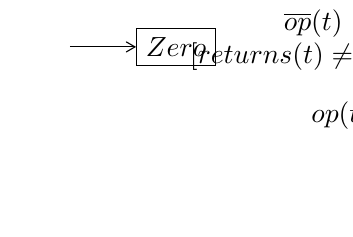
\begin{tikzpicture}[>= angle 60, xscale = 0.9, yscale = 0.44]
\draw (0,0) node[draw] (zero) {$\sm{Zero}$};
\draw[->] (zero) ++ (-1.5, 0) -- (zero);
\loopAbove(zero){$\begin{array}{c}
  \overline\op(\sm t) \\ {[\sm{returns(t)} \ne \sm{None}]}
  \end{array}$}
%
\draw (0,-4) node[draw] (one) {$\sm{One}(\sm t_1, \sm{x}_1)$};
\draw[->] (zero) .. controls ++(0.3,-2) .. 
  node[right] {$\sm{op}(\sm t_1, \sm{x}_1)$} (one); 
%
\draw[->] (one) .. controls ++(-0.3,2) .. 
  node[left] {$\sm{op}(\sm t_2, \sm x_2)$} (zero);
\end{tikzpicture}%
\end{minipage}
},]
We now consider the homogeneous case.  For simplicity, we describe the binary
case; synchronisations of more than two operation executions are handled
similarly.  Suppose we have a synchronisation object with a single operation
%\protect\SCALA{def op(x: A): B}.  
{\bfseries\scalastyle def}~{\scalastyle op(x: A): B}.  
All executions of~|op| have to be treated similarly,
so we associate \emph{each} with two operations |op| and $\overline{\sm{op}}$
of the specification object.  The specification object is below, and encodes
the automaton on the right.
The second execution of |op| in any synchronisation (from the |One| state of the
automaton) writes the results of the execution into the |returns| array.
Each execution of $\overline{\sm{op}}$ returns the stored value.
\end{window}
%
%% \begin{trivlist}
%% \item[]
%\begin{minipage}{92mm}
\begin{scala}
class TwoStepHomoLinSpec{
  private var state: State = Zero
  private val returns = new Array[Option[B£\s1£]](NumThreads)
  for(t <- 0 until NumThreads) returns(t) = None
  def op(t: ThreadID, x: A): Unit = {
    require(returns(t) == None)
    state match{
      case Zero => state = One(t, x)
      case One(t£\s1£, x£\s1£) => 
        val (y£\s1£, y£\s2£) = SyncSpec.sync(x£\s1£, x) 
        returns(t£\s1£) = Some(y£\s1£); returns(t) = Some(y£\s2£); state = Zero
    }
  }
  def £$\overline{\sm{op}}$£(t: ThreadID): B = {
    require(state.isInstanceOf[Zero] && returns(t).isInstanceOf[Some])
    val Some(y) = returns(t); returns(t) = None; y
  }
}
\end{scala}


%%%%%%%%%%%%%%%%%%%%%%%%%%%%%%%%%%%%%%%%%%%%%%%%%%%%%%% Mixed arity

Recall that some operations have multiple modes of synchronisations: different
executions of the operation may have synchronisations with different arities.
For example, in a timeout channel, an execution of the |send| and |receive|
operations may synchronise with an execution of the other operation, or may
timeout corresponding to a unary synchronisation.

\begin{window}[0,r,{
\begin{minipage}{52.9mm}
\begin{tikzpicture}[>= angle 60, xscale = 0.9, yscale = 0.44]
\draw (0,0) node[draw] (zero) {$\sm{Zero}$};
\draw[->] (zero) ++ (-1.5, 0) -- (zero);
% self-loop on Zero
\loopAbove(zero){$\begin{array}{@{}c@{}}
      \receive()\::\sm{None}, \\ 
      \overline{\send}(\sm t)\::\sm{true} [\sm{returns(t)} \ne \sm{None}]
    \end{array}$}
%%%%%% One
\draw (0,-5) node[draw] (one) {$\sm{One}(\sm t, \sm{x})$};
\draw[->] (zero) .. controls ++(0.3,-2.5) .. 
  node[right] {$\send(\sm t, \sm{x})$} (one); 
\draw[->] (one) .. controls ++(-0.3,2.5) .. 
  node[left] {$\begin{array}[t]{@{}r@{}}
   \receive()\::\sm{Some(x)}, \\ \overline{\send}(\sm t)\::\sm{false}
    \end{array}$} (zero);
\end{tikzpicture}
\end{minipage}
},] 
The figure to the right gives the automaton for a timeout
channel, where we treat $\send$ as corresponding to $\op_1$ (we omit concrete
code in the interests of brevity).  The automaton is similar to that for a
standard channel.  The |receive| operation can happen from either state: if it
happens from the |One| state, then a synchronisation has occurred and the
execution returns a value of the form |Some(x)|; but if it happens from the
|Zero| state, there has been no corresponding |send|, and so the execution
returns~|None|, indicating a timeout.  Likewise, the $\overline{\send}$
operation can happen from either state; if it happens from the |Zero| state,
then a synchronisation has occurred and the execution returns |true|; but if
it happens from the |One| state, there has been no corresponding |receive|,
and so the execution returns~|false|, indicating a timeout.
\end{window}



%%%%%%%%%%%%%%%%%%%%%%%%%%%%%%%%%%%%%%%%%%%%%%%%%%%%%%% Stateful

We now consider stateful specification objects.  In general, we can simply
augment the |Zero| and |One| states of the automaton to include the state of
the specification object.  Different transitions may be available
based upon that state.  However, it can be clearer and simpler to introduce
different named states into the automaton.

The figure below gives the specification automaton for a closeable channel.
%
%\begin{figure}
\begin{center}
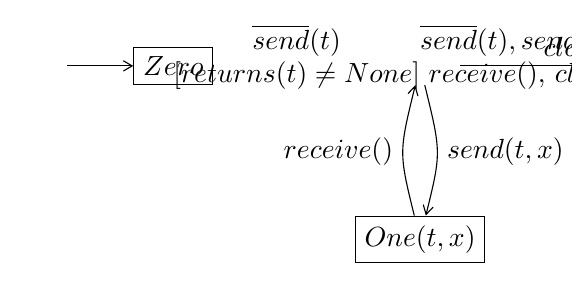
\begin{tikzpicture}[>= angle 60, xscale = 0.9, yscale = 0.44]
\draw (0,0) node[draw] (zero) {$\sm{Zero}$};
\draw[->] (zero) ++ (-1.5, 0) -- (zero);
% self-loop on Zero
\loopAbove(zero){$\begin{array}{@{}c@{}}
  \overline{\send}(\sm t) \\ {[\sm{returns(t)} \ne \sm{None}]}
  \end{array}$}
%%%%%% One
\draw (0,-5) node[draw] (one) {$\sm{One}(\sm t, \sm{x})$};
\draw[->] (zero) .. controls ++(0.3,-2.5) .. 
  node[right] {$\send(\sm t, \sm{x})$} (one); 
\draw[->] (one) .. controls ++(-0.3,2.5) .. 
  node[left] {$\receive()$} (zero);
%%%%%% Closed
\draw (4.5,0) node[draw] (closed) {$\sm{Closed}$};
\draw[->] (zero) -- node[above] {$\sm{close}$} (closed);
% self-loop on closed
\loopAbove(closed){$\begin{array}{@{}c@{}}
      %% \overline{\send}(\sm t) [\sm{returns(t)} \ne \sm{None}], \\
      %% \send(\sm t), \, \receive(), \, \sm{close} 
      \overline{\send}(\sm t), \send(\sm t, \sm x), \\ \receive(), \, \sm{close}() 
    \end{array}$} 
\end{tikzpicture}
\end{center}
%% \caption{Automaton for capturing two-step linearisation for a closeable
%%   channel.}
%% \label{fig:two-step-closeable-chan}
%% \end{figure}
%
The automaton has an additional state, |Closed|,
corresponding to the channel being closed.  All executions are unary
synchronisations in this state.  This automaton represents a simplification
over the general approach discussed above: we do not need two separate states
after closing.  Note that a $\overline{\send}(\sm t)$ transition from the
|Closed| state may succeed if the corresponding synchronisation happened
before the channel was closed, in which case $\sm{returns(t)} \ne \sm{None}$.

%%%%%%%%%%

\subsection{The general construction}
\label{ssec:relating-general}

We now give a general construction to show how two-step linearisation can
capture synchronisation linearisation. 
%
Fix a synchronisation object~|SyncObj|, a synchronisation specification object
|SyncSpec|, and synchronisation abstraction function~$\A$.  Let the operations
of the |SyncObj| be
\begin{scala}
  def op£\s i£(x: A£\s i£): B£\s i \qquad for $i = 1,\ldots,n$.£
\end{scala}

The two-step linearisation tester has operations $\op_i$ and
$\overline\op_i$ for $i = 1,\ldots,n$. 
%
The idea is that for a mapping 
\[
\seq{\op_{i_i}(x_1), \ldots, \op_{i_a}(x_a)}
  \mapsto \sync(x_1,\ldots,x_a)  \in \A,
\]
corresponding to a synchronisation of arity~$a$, is linearised in the
following order:
\begin{enumerate}
\item $\op_{i_1},\ldots,\op_{i_a}$, in order;

\item $\overline\op_{i_i}$, for some~$i$, which  calls
  |SyncSpec.sync|$(x_1,\ldots,x_a)$, and stores the results for other threads;

\item The remaining $\overline\op_{i_j}$, in some order, which  retrieve
  their results.
\end{enumerate}
%
No other operation occurs between the start of stage~1 until after
stage~2; but other operations may occur during stage~3.

During stage~1, the two-step linearisabilty tester  records the prefix of
$\seq{\op_{i_i}(x_1), \ldots, \op_{i_a}(x_a)}$ performed so far.  This is done
by defining a case class |Op|$_i$ corresponding to each such
operation~|op|$_i$, as at the top of Figure~\ref{fig:schema}.
%
%% \begin{scala}
%% trait Op
%% case class Op_i(t: ThreadID, x: A_i) £\quad for $i = 1,...,n$.£
%% type State = List[Op]
%% \end{scala}
%
The following function maps such a sequence to the corresponding sequence of
operations, for use with~$\A$.
\begin{eqnarray*}
\opsFor(state) &  = & \seq{\op_j(x_j) \midd \sm{Op}_j(t_j,x_j) \leftarrow state}.
\end{eqnarray*}

A schema (using pseudo-Scala) for the general construction is in
Figure~\ref{fig:schema}.  The variable~|state| records the sequence of
|op|$_i$ linearised so far: this satisfies an invariant that it is a prefix of
an element of $\dom \A$.  For each thread~|t|,\, |returns(t)| stores the value
to be returned by~|t| as part of its most recent uncompleted synchronisation,
if any. % , where $B = \bigcup\nolimits_{i = 1,\ldots,n} \sm B_i$.

%%%%%

\begin{figure}
\begin{scala}
trait Op
case class Op£$_i$£(t: ThreadID, x: A£$_i$£) //  for £$i = 1,...,n$.£
type State = List[Op]
type B = £$\bigcup\nolimits_{i = 1,\ldots,n} \sm B_i$£

class TwoStepLinSpec{
  private var state: State = List()
  private val returns = Array.fill[Option[B]](NumThreads)(None) 

  def op£\s i£(t: ThreadID, x: A£\s i£): Unit = { // for £$i = 1,...,n$£.
    require(£$\exists ops \in \dom \A \spot \opsFor(\sm{state}) \cat \seq{\op_i(x)} \prefix ops$£)
    state = state :+  Op£\s i£(t,x) 
  }

  def £$\overline\op_i$£(t: ThreadID): B£\s i£ = { // for £$i = 1,...,n$£.
    if(£$\opsFor(\sm{state}) \in \dom \A$£){
      val (y£\s 1£,...,y£$_{\ss a}$£) = SyncSpec.£$\A(\opsFor(\sm{state}))$£
      for(m <- 1 to a) returns(State(m).t) = Some(y£$_{\ss m}$£)
      state = List()
    }
    else (require(state == List() && returns(t).isInstanceOf[Some])
    val Some(y) = returns(t); returns(t) = None; y
  }
}
\end{scala}
\caption{A schema for the general construction of a two-step linearisability
  tester.} 
\label{fig:schema}
\end{figure}

%%%%%

The operation $\op_i$ appends an appropriate |Op|$_i$ object to~|state|.  The
precondition ensures that |state| still corresponds to a prefix of an element
of $\dom \A$.  

The operation $\overline\op_i$ proceeds as follows.  In the case that |state|
corresponds to an element of $\dom \A$, it calls the corresponding operation
on |SyncSpec|, stores each result in the corresponding entry of |returns|, and
resets |state|.  Otherwise, it requires that some other operation has called
the operation on |SyncSpec|, and that |state| holds its initial value.  In
either case, the operation retrieves and clears its result from the
appropriate entry in~|returns|.

It is then straightforward to check that operations of |TwoStepLinSpec| can be
linearised only as described earlier.  The proof that two-step linearisability
corresponds to synchronisation linearisability is then much as in the proof
for the binary case in Proposition~\ref{prop:two-step-lin}. 

Figure~\ref{fig:schema} uses preudo-Scala.  For a concrete implementation, we
need a separate implementation of $\op_i$ and $\overline\op_i$ for each~$i$.
Then each calculation involving~$\A$ can be implemented directly, for example
using a case analysis.



%% We believe that these techniques can be adapted to all the other
%% synchronisation objects we have considered.

%% These techniques can be adapted to all other synchronisation objects of the
%% form we are considering.  We sketch a generic approach; we omit the details
%% because they are fiddly and uninteresting.  For each operation |op|$_i$ of the
%% synchronisation object, the two-step linearisation specification object
%% includes operations $\op_i$ and $\overline{\op}_i$.  For each maplet
%% $\seq{\op_{i_i}(x_1), \ldots, \op_{i_a}(x_a)} \mapsto \sync(x_1,\ldots,x_a)$
%% in the synchronisation abstraction function, the two-step linearisation
%% specification object performs operations as follows: (1)~$\op_{i_i}(x_1),
%% \ldots, \op_{i_a}(x_a)$, in that order; (2)~$\overline\op_{i_i}$, for
%% some~$i$, which calls \sync\ on the synchronisation linearisation object and
%% stores the results for other threads; (3)~the remaining $\overline\op_{i_j}$,
%% in some order, which retrieve their results.

\section{Linearisability testing}
\label{sec:lin-testing}

In the following two sections, we describe techniques for testing whether the
implementation of a synchronisation object is synchronisation linearisable
with respect to a synchronisation specification object.
%
The techniques are influenced by the techniques for testing (standard)
linearisation~\cite{wing-gong,gavin:lin-testing}, so we begin by sketching
those techniques.

The idea of linearisability testing is as follows.  We run several
\emph{worker threads}, performing operations (typically chosen randomly) upon
the concurrent datatype that we are testing, and logging the calls and
returns.  More precisely, a thread that performs a particular
operation~$\sm{op}^i(x)$: (1) writes $\call.\sm{op}^i(x)$ into the log;
(2)~performs $\sm{op}(x)$ on the synchonisation object, obtaining result~$y$,
say; (3)~writes $\return.\sm{op}^i \:: y$ into the log.  Further, the logging
associates each operation execution with an execution $\sm{op}(x)$ of the
corresponding operation on the specification object.

Once all worker threads have finished, we can use an algorithm to test whether
the history is linearisable with respect to the specification object.  The
algorithm searches for an order to linearise the executions, consistent with
the log, and such that the order represents a legal history of the
corresponding executions on the specification object.
See~\cite{wing-gong,gavin:lin-testing} for details of several algorithms.
All these algorithms assume that the specification object is deterministic.

This process can be repeated many times, so as to generate and analyse many
histories.  Our experience is that the technique works well.  It seems
effective at finding bugs, where they exist, typically within a few seconds;
for example, we used it to find an error in the concurrent priority queue
of~\cite{faulty-pri-queue}, which we believe had not previously been
documented.  Further, the technique is easy to use: we have taught it to
undergraduate students, who have used it effectively.

This testing concentrates upon the safety property of
linearisation, rather than liveness properties such as deadlock-freedom.
However, if the concurrent object can deadlock, it is likely that the testing
will discover this.  Related to this point, it is the responsibility of the
tester to define the worker threads in a way that all executions will
eventually return, so the threads terminate.  For example, consider a partial
stack where a |pop| operation blocks while the stack is empty; here, the
tester would need to ensure that threads collectively perform at least as many
|push|es as |pop|s, to ensure that each |pop| does eventually return.

Note also that there is potentially a delay between a worker thread writing the
$\call$ event into the log and actually calling the operation; and likewise
there is potentially a delay between the operation returning and the thread
writing the $\return$ event into the log.  However, these delays do not
generate false errors: if a history without such delays is linearisable, then
so is a corresponding history with delays.  We believe that it is essential
that the technique does not give false errors: an error reported by testing
should represent a real error; testing of a correct implementation should be
able to run unsupervised, maybe for a long time.  Further, our experience is
that the delays do not prevent the detection of bugs when they exist (although
might require performing the test more times).  This means that a failure to
find any bugs, after a large number of tests, can give us good confidence in
the correctness of the concurrent datatype.

%%%%%%%%%%%%%%%%%%%%%%%%%%%%%%%%%%%%%%%%%%%%%%%%%%%%%%%

\section{Adapting the linearisability framework}
\label{sec:testing-hacking}

In this section we investigate how to use the existing linearisation testing
framework for testing synchronisation linearisation, using the ideas of
Section~\ref{sec:relating}.  We require the synchronisation specification
object to be deterministic, reflecting the fact that the linearisation
testing framework requires its specification object to be deterministic.  

This is not a use for which the framework was intended, so we consider it a
hack.  However, it has the advantage of not requiring the implementation of
any new algorithms.  (We do not consider progressibility in this section.)

%% Recall, from the introduction of Section~\ref{sec:relating}, that a
%% straightforward approach won't work.  Instead 

We adapt the idea of two-step linearisation from Section~\ref{sec:relating}.
We start by considering the case of binary heterogeneous synchronisation.  We
aim to obtain a log history that can be tested for (standard) linearisation
against |TwoStepLinSpec|.

As with standard linearisability testing, we run several worker threads,
calling operations on the synchronisation object, and logging the calls and
returns.
%
\begin{itemize}
\item A thread~$t_1$ that performs the concrete operation~$\op_1(x_1)$:
  (1)~writes $\call.\sm{op}_1^{i_1}(x_1)$ into the log, associating it with a
  corresponding execution $\op_1(t_1, x_1)$ on the specification object;
  (2)~performs $\op_1(x_1)$ on the synchonisation object, obtaining
  result~$y_1$, say; (3)~writes $\return.\op_1^{i_1} \:: ()$ into the log;
  (4)~writes $\call.\overline{\op}_1^{i_1}()$ into the log, associating it
  with a corresponding execution $\overline{\op}_1(t)$ on the specification
  object; (5)~writes $\return.\overline{\op}_1^{i_1} \:: y_1$ into the log.

\item A thread~$t_2$ that performs operation~|op|\s2, acts as for standard
  linearisability testing.  It: (1)~writes $\call.\sm{op}_2^{i_2}(x_2)$ into
  the log, associating it with a corresponding execution $\op_2(x_2)$ on the
  specification object; (2)~performs $\op_2(x_2)$ on the synchonisation
  object, obtaining result~$y_2$, say; (3)~writes $\return.\op_2^{i_2} \::
  y_2$ into the log
\end{itemize}
%
The top half of Figure~\ref{fig:twostep-timeline} illustrates a possible run,
containing a single synchronisation, together with the log history.

\begin{figure}
\begin{center}
\def\y{-1.4} % op_2 y-coord
\def\ySLin{-2.5} % sync-lin y-ccord
\def\yLin{-3.6} % linearisation y-coord
\begin{tikzpicture}%[yscale = 1.4]
\bulletAt(-0.6,0){$\call.\op_1(x_1)$};
\draw[|-|] (0.0,0) -- node[above] {$\op_1(x_1)\::y_1$} (2.5,0);
\bulletAt(3.1,0){$\return.\op_1$};
\bulletAt(4.7,0){$\call.\overline{\op}_1$};
\bulletAt(6.5,0){$\return.\overline{\op}_1\::y_1$};
%
\bulletAt(-0.3,\y){$\call.\op_2(x_2)$};
\draw[|-|] (0.4,\y) -- node[above]{$\op_2(x_2)\::y_2$} (2.7,\y);
\bulletAt(3.5,\y){$\return.\op_2\::y_2$};
%
\draw (-2,\ySLin) node{$h_s$};
\crossAt(1.4,\ySLin){$\sync(x_1,x_2)\::(y_1,y_2)$};
%
\draw (-2,\yLin) node{$h_{2s}$:};
\draw(1.2,\yLin) \X; 
\draw(0.5,\yLin-0.4) node{\footnotesize $\op_1(t_1,x_1)$};
\draw(1.6,\yLin) \X;
\draw(2.3,\yLin-0.4) node{\footnotesize $\op_2(x_2)\::y_2$};
%% \crossAt(0.5,\yLin){$\op_1(t_1,x_1)$};
%% \crossAt(2.3,\yLin){$\op_2(x_2)\::y_2$};
\crossAt(5.5,\yLin){$\overline{\op}_1(t_1)\::y_1$};
\end{tikzpicture}
\end{center}
\caption{Illustration of two-step linearisation testing.  The operation
  executions are represented by the horizontal lines with labels above
  (denoted ``$h$'' in Proposition~\ref{prop:twostep-testing}).  The log
  entries are represented by the bullets with labels below (denoted ``$h_l$''
  in Proposition~\ref{prop:twostep-testing}).  Linearisation points are
  represented by crosses with labels below: the penultimate row, labelled
  ``$h_s$'', is a synchronisation linearisation; the bottom row, labelled
  ``$h_{2s}$'', is a linearisation of the two-step synchronisation object.
  Execution identifiers and null arguments and returns are omitted, for
  clarity.}
\label{fig:twostep-timeline}
\end{figure}

%%%%%

Once all threads have finished, we test whether the log history is
linearisable (i.e.~standard linearisation) with respect to |TwoStepLinSpec|
from Section~\ref{sec:relating}.  Figure~\ref{fig:twostep-timeline} gives an
example linearisation, denoted~$h_{2s}$.

Note that we have three related concepts here: (1)~synchronisation
linearisation of the concrete history of operation executions with respect to
|SyncSpec|; (2)~two-step linearisation of the concrete history with respect
to~|TwoStepLinSpec|; and (3)~linearisation of the log history with respect
to~|TwoStepLinSpec|.  Proposition~\ref{prop:two-step-lin} shows that the first
two of these are equivalent.  We need to show that these imply~(3), so the
technique does not give false errors.  (The converse might not hold, because
of delays in writing to the log.)

Since the linearisation algorithm receives  a log history, rather
than a concrete history, we need to describe the relationship.  
%% The following definition captures that a log history~$h_l$ might arise from a
%% concrete history~$h$, using the logging strategy described above.
%
\begin{definition}
Let $h$ be a complete history of a binary heterogeneous synchronisation
object, and let $h_l$ be a log history for the same object.  We say that the
two histories \emph{correspond} if there is some way of interleaving them such
that
%
\begin{itemize}
\item Each $\call.\op_1^{i_1}(x_1)$, from $h_l$, precedes the call and return
  of~$\op_1^{i_1}(x_1)\::y_1$ from~$h$, which precede $\return.\op_1^{i_1} \::
  ()$, $\call.\overline{\op}_1^{i_1}()$ and $\return.\overline{\op}_1^{i_1}
  \:: y_1$, from~$h_l$, in that order.

\item Each $\call.\op_2^{i_2}(x_2)$, from $h_l$, precedes the call and return
  of~$\op_2^{i_2}(x_2)\::y_2$ from~$h$, which precede $\return.\op_2^{i_2}
  \:: y_2$, from~$h_l$.
\end{itemize}
\end{definition}

\begin{prop}
\label{prop:twostep-testing}
Let $h$ be a complete history of a binary heterogeneous synchronisation
object, and let $h_l$ be a corresponding log history for the same object.  Let
|SyncSpec| be a synchronisation specification object, and |TwoStepSyncSpec|
the corresponding two-step synchronisation specification object, constructed
as in Section~\ref{sec:twoStepLinSpec}.  Suppose $h$ is
synchronisation-linearisable with respect to |SyncSpec|.  Then $h_l$ is
linearisable with respect to |TwoStepSyncSpec|.
\end{prop}
%
\begin{proof}
Since $h$ is synchronisation-linearisable, there is a legal history~$h_s$ of
|SyncSpec| such that $h_s$ is a synchronisation linearisation of $h$.
Consider the interleaving of $h_s$ and~$h$, that demonstrates this, and
interleave $h_l$ with it, consistent with the interleaving of~$h$ and~$h_l$
that demonstrates that they correspond.  Figure~\ref{fig:twostep-timeline}
illustrates such an interleaving.

We build a history~$h_{2s}$ of~|TwoStepSyncSpec|, and interleave it with~$h_l$
as follows.  In the interleaving of the previous paragraph, replace each event
$\sync^{i_1,i_2}(x_1,x_2)\::(y_1,y_2)$ (from~$h_s$) by immediately consecutive
events~$\op_1^{i_1}(x_1)\::()$ and $\op_2^{i_2}(x_2)\::y_2$, and add
$\overline{\op}_1^{i_1}()\::y_1$ between $\call.\overline{\op}_1^{i_1}()$ and
$\return.\overline{\op}_1^{i_1} \:: y_1$ (from~$h_l$).  Again,
Figure~\ref{fig:twostep-timeline} illustrates such an interleaving.  This is a
legal history of~|TwoStepSyncSpec|, by
Lemma~\ref{lem:TwoStepLinSpec-histories}.  Further, each event of~$h_{2s}$ is
between the corresponding $\call$ and $\return$ events of~$h_l$, by
construction.  Hence $h_{2s}$ is a linearisation of~$h_l$.
\end{proof}

%%%%%%%%%%%%%%%%%%%%%%%%%%%%%%%%%%%%%%%%%%%%%%%%%%%%%%%

%% \subsection{OLD VERSION}

%% Note there might be delays involved in writing to the log, so that the log
%% history does not correspond precisely to the history of operation calls and
%% returns.  We show that the approximation serves our purposes.

%% Consider a history~$h$ of the synchronisation object, and suppose, for the
%% moment, there are no delays in logging, i.e.:\ (1)~the $\call.\op_1$ and
%% $\call.\op_2$ events happen immediately before the actual calls; (2)~the
%% $\return.\op_2$ events happen immediately after the return of~$\op_2$; and
%% (3)~the $\call.\overline\op_1$ and $\return.\overline\op_1$ events happen
%% immediately after the return of $\op_1$ --- in each case with no intervening
%% events.  Then the log history is linearisable with respect to |TwoStepLinSpec|
%% if and only if the history~$h$ is two-step linearisable with respect to
%% |TwoStepLinSpec|.  But Proposition~\ref{prop:two-step-lin} then shows that
%% this holds if and only if $h$ is synchronisation linearisable.  In particular,
%% this shows that errors are detected providing the logging is fast enough.

%% We now show that delays in logging do not introduce false errors.  Consider a
%% history~$h$ that is synchronisation linearisable, and consider the
%% corresponding log history~$h_l$.  Now build a history~$h'$ so that each
%% operation is extended so that: (1)~each call of~$\op_1$ or~$\op_2$ is
%% immediately before the $\call.\op_1$ or $\call.\op_2$ event in~$h_l$; (2)~each
%% return of~$\op_1$ is immediately after the $\return.\overline\op_1$ event
%% in~$h_l$; and (3)~each return of~$\op_2$ is immediately after the
%% $\return.\op_2$ event in~$h_l$.  This construction is illustrated below for
%% the two types of operation.
%% %
%% \begin{center}
%% \begin{tikzpicture}[xscale = 1.0, yscale = 1.0]
%% \draw (-2.0,0) node{$h$:};
%% \draw (-2.0,-1) node{$h_l$:};
%% \draw (-2.0,-2.3) node{$h'$:};
%% % op_1^1
%% \draw[|-|] (0,0) -- node[above] {$\sm{op}_1(x_1)\::y_1$} (1,0);
%% \bulletAt(-0.2,-0.8){$\call.\sm{op}_1$}
%% \bulletAt(1.2,-0.8){$\return.\sm{op}_1$}
%% \bulletAt(2.7,-0.8){$\call.\overline{\op}_1$}
%% \bulletAt(4.2,-0.8){$\return.\overline{\op}_1$}
%% \draw[|-|] (-0.4,-2.3) -- node[above] {$\sm{op}_1(x_1)\::y_1$} (4.4,-2.3);
%% %%%%%
%% \draw[|-|] (7.0,0) -- node[above] {$\sm{op}_2(x_2)\::y_2$} (8,0);
%% \bulletAt(6.8,-0.8){$\call.\sm{op}_2$}
%% \bulletAt(8.2,-0.8){$\return.\op_2$}
%% \draw[|-|] (6.6,-2.3) -- node[above] {$\sm{op}_2(x_2)\::y_2$} (8.4,-2.3);
%% \end{tikzpicture}
%% \end{center}
%% %
%% Now $h$ is synchronisation linearisable; and hence $h'$ is also (since each
%% operation in $h'$ is an extension of the corresponding operation in~$h$).  But
%% then Proposition~\ref{prop:two-step-lin} implies that $h'$ is two-step
%% linearisable with respect to |TwoStepLinSpec|.  Hence $h_l$ is linearisable
%% with respect to |TwoStepLinSpec|, by construction.

This approach generalises to non-binary synchronisations, homogeneous
synchronisations, and stateful specification objects as in
Section~\ref{ssec:relating-variations}.


As with standard linearisation, the tester needs to define the worker threads
so that all executions will eventually return, i.e.~so that each will be able
to synchronise.  For a binary heterogeneous synchronisation with no
precondition, we can achieve this by half the threads calling one operation,
and the other half calling the other operation (with the same number of calls
by each).  For a binary homogeneous synchronisation, this approach might not
work if every worker does more than one operation: one worker might end up
with two operations to perform, when all others have terminated; instead, we
arrange for an even number of workers to each perform a single operation.


%%%%%%%%%%%%%%%%%%%%%%%%%%%%%%%%%%%%%%%%%%%%%%%%%%%%%%%

\paragraph{Variable-arity synchronisations}

It turns out that it is not, in general, possible to capture variable-arity
synchronisations using this technique, in particular where the arity of a
synchronisation depends upon the relative timing of executions, as opposed to
the state of the specification object.  This is a result of two things: that
the logging of operations, in particular the $\overline{\op}_1$, can be
arbitrarily delayed; and that it can be nondeterministic whether or not two
executions synchronise, which is at odds with the fact that each operation on
the specification object needs to be deterministic.

To illustrate this point, consider a timeout channel.  Without loss of
generality, let the |send| operation correspond to $\op_1$, and the
|receive| operation correspond to~$\op_2$.

The top-half of Figure~\ref{fig:two-step-timeout-channel} gives a
timeline illustrating a successful |send(3)| and |receive|.  This
corresponds to the history
\[
\seq{ \send(3)\::(),\; \receive()\::\sm{Some}(3),\; 
  \overline{\send}()\::\sm{true} }
\]
of the specification object.

%%%%%%%%%%

\begin{figure}
\begin{center}
\def\yLin{-2.5} % y-coord for linearisation
\begin{tikzpicture}[xscale = 0.9]
\bulletAt(-0.4,0){$\call.\send(3)$};
\draw[|-|] (0,0) -- node[above] {$\send(3)\::()$} (1.6,0);
\bulletAt(2.0,0){$\return.\send$};
%
\bulletAt(3.9,0){$\call.\overline{\send}$};
\bulletAt(6.2,0){$\return.\overline{\send}\::\sm{true}$};
%
\bulletAt(-0.5,-1.5){$\call.\receive\qquad$};
\draw[|-|] (0.3,-1.5) -- 
  node[above] {$\receive()\::\sm{Some}(3)$} (1.9,-1.5);
\bulletAt(2.8,-1.5){\ $\qquad\qquad\return.\receive\::\sm{Some(3)}$};
%
\draw(0.7,\yLin) \X; 
\draw(-0.1,\yLin-0.4) node{\footnotesize $\send(3)\::()$};
\draw(1.1,\yLin) \X;
\draw(2.6,\yLin-0.4) node{\footnotesize $\receive()\::\sm{Some}(3)$};
%% \crossAt(0.7,-3){$\send(3)\::()$}
%% \crossAt(1.5,-3){$\receive()\::\sm{Some}(3)$}
\crossAt(5.5,\yLin){$\overline{\send}\::\sm{true}$}
%
\draw (-2.2,-3.6) -- ++(12.4,0); 
\end{tikzpicture}

%%%%%%
%\hfil\hfil
\medskip

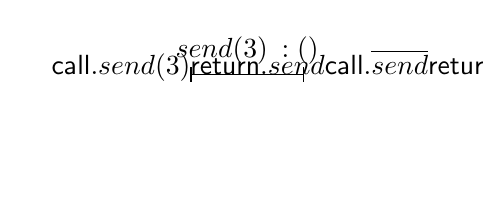
\begin{tikzpicture}[xscale = 0.9]
\bulletAt(-0.4,0){$\call.\send(3)$};
\draw[|-|] (0,0) -- node[above] {$\send(3)\::()$} (1.6,0);
\bulletAt(2.0,0){$\return.\send$};
%
\bulletAt(7.1,0){$\call.\overline{\send}$};
\bulletAt(9.4,0){$\return.\overline{\send}\::\sm{false}$};
%
\bulletAt(2.5,-1.5){$\call.\receive\qquad$};
\draw[|-|] (3.3,-1.5) -- 
  node[above] {$\receive()\::\sm{None}$} (4.9,-1.5);
\bulletAt(5.8,-1.5){\ $\qquad\qquad\return.\receive\::\sm{None}$};
%
\crossAt(0.8,\yLin){$\send(3)\::()$};
\crossAt(3.9,\yLin){$\receive()\::\sm{Some}(3)$};
\crossAt(8.2,\yLin){$\overline{\send}\::\sm{true}$}
%% \draw[|-|] (0,-3.5) -- node[above] {$\send(3)\::()$} (1.6,-3.5);
%% \crossAt(0.7,-3.5){$\send(3)\::()$}
%% %
%% \draw[|-|] (2.2,-5) -- 
%%   node[above] {$\receive()\::\sm{None}$} (3.8,-5);
%% \crossAt(3.4,-5){$\receive()\::\sm{Some}(3)$}
%% %
%% \draw[|-|] (4.0,-3.5) -- node[above] 
%%   {$\overline{\send}(3)\::\sm{false}$} (5.6,-3.5);
%% \crossAt(4.8,-3.5){$\overline{\send}(3)\::\sm{true}$}
\end{tikzpicture}
\end{center}
\caption{Figure showing why two-step linearisation cannot be used for a
  timeout channel.  Conventions are as in Figure~\ref{fig:twostep-timeline}.}
\label{fig:two-step-timeout-channel}
\end{figure}

%%%%%%%%%%

The bottom-half side of Figure~\ref{fig:two-step-timeout-channel} gives a
timeline illustrating an unsuccessful |send(3)| and |receive|, and where the
logging of $\overline{\send}$ is delayed.  None of the executions overlap, so
they must necessarily be linearised in the same order as in the previous
history.  The specification object is deterministic, so the operations must
return the same results as in the previous history.  But, in the cases of
$\receive$ and $\overline{\send}$, those returned values, |Some(3)| and
|true|, do not agree with the corresponding values in the log history, |None|
and |false|.  Hence the history would be flagged as an error, despite being
valid.

The difference between this situation and the discussion in
Section~\ref{ssec:relating-variations} is that the logging of
operations, in particular the $\overline{\send}$, can be arbitrarily delayed.
However, in the earlier section we allowed the $\overline{\send}$ anywhere
within the corresponding concrete operation.  This means that a history like
in the bottom-half of Figure~\ref{fig:two-step-timeout-channel} could be
linearised by the history
\[
\seq{ \send(3)\::(),\; \overline{\send}(3)\::\sm{false},\;
  \receive()\::\sm{None} }
\]
of the two-step specification object.  Here the operations take place in a
different order than for Figure~\ref{fig:two-step-timeout-channel}, and so
this is consistent with a deterministic specification object.

A similar problem arises with a timeout exchanger.

%\framebox{Explain how it can be done.}

We have investigated an alternative approach, which involves worker threads
adapting their logging behaviour based on the outcome of their operations.
For the timeout channel:
\begin{itemize}
\item A thread that sends a value~$x$: (1)~writes $\call.\send^{i_1}(x)$ into
  the log; (2)~performs $\send(x)$ on the channel; (3)~writes
  $\return.\send^{i_1} \:: ()$ into the log; (4)~if the send is successful,
  associates the log entries with an operation $\send(x)$ on the specification
  object, and otherwise associates them with an operation $\sm{sendFail}(x)$;
  (5)~if the send is successful, writes $\call.\overline{\send}^{i_1}()$ and
  $\return.\overline{\send}_1^{i_1} \:: ()$ into the log, associating them
  with an operation $\overline{\send}()$ on the specification object (and
  otherwise does nothing).

%%     (6)~writes $\return.\overline{\send}_1^{i_1} \:: ()$ into the log

%% then:
%%   \begin{itemize}
%%   \item if the send is successful: (4) associates the log entries with an
%%     operation $\send(x)$ on the specification object; (5)~writes
%%     $\call.\overline{\send}^{i_1}()$ into the log, associating it with a
%%     corresponding execution $\overline{\send}()$ on the specification object;
%%     (6)~writes $\return.\overline{\send}_1^{i_1} \:: ()$ into the log.

%%   \item if the send is unsuccessful: (4)~associates the log entries with an
%%     operation $\sm{sendFail(x)}$ on the specification object (and does not
%%     perform the second step).
%%   \end{itemize}

\item A thread that performs a receive: (1)~writes $\call.\receive^{i_2}$ into
  the log; (2)~performs $\receive$ on the channel, receiving result~$r$, say;
  (3)~writes $\return.\receive^{i_1} \:: r$ into the log; (4)~if the receive
  was successful, associates the log entries with an operation |receive| on
  the specification, and otherwise associates them with an
  operation $\sm{receiveFail}$.
\end{itemize}



\begin{window}[0,r,{
\begin{minipage}{48.5mm}
\begin{tikzpicture}[>= angle 60]
\draw (0,0) node[draw] (zero) {$\sm{Zero}$};
\draw[<-] (zero) -- ++ (-1.5,0);
\loopRight(zero){$
%% \draw[->] (zero) .. controls ++(1.5,0.4) and (1.5,-0.4) .. node[right] {$
  \begin{align} 
  \sm{sendFail}, \\ \overline{\send}, \\ \sm{receiveFail}
  \end{align}$}% (zero);
%
\draw (0,-2) node[draw] (one) {$\sm{One}(\sm{x})$};
\draw[->] (zero) .. controls ++(0.3,-1) .. node[right] {$\sm{send(x)}$} (one); 
\draw[->] (one) .. controls ++(-0.3,1) .. 
  node[left] {$\begin{align}\sm{receive}\::\\ \quad\sm{Some(x)}\end{align}$} (zero);
\end{tikzpicture}
\end{minipage}
},] 
The specification object then encodes the automaton to the right.
Thus a successful synchronisation is linearised by the sequence $\send(\sm x)$,
$\receive\::\sm{Some(x)}$, $\overline{\send}$, with the former two events
consecutive, as for other binary heterogeneous synchronisations.  Unsuccessful
sends and receives are each linearised by a single event.
\end{window}

%%%%%%%%%%%%%%%%%%%%%%%%%%%%%%%%%%%%%%%%%%%%%%%%%%%%%%%

%% The specification object then encodes the automaton below. 
%% %% \begin{window}[0,r,{
%% %% \begin{minipage}{73mm}
%% \begin{center}
%% \begin{tikzpicture}[>= angle 60]
%% \draw (0,0) node[draw] (zero) {$\sm{Zero}$};
%% \draw[<-] (zero) -- ++ (-1.5,0);
%% \loopAbove(zero){$
%% %% \draw[->] (zero) .. controls ++(1.5,0.4) and (1.5,-0.4) .. node[right] {$
%%   \begin{array}{c} 
%%   \sm{sendFail}, \overline{\send}, \\ \sm{receiveFail}
%%   \end{array}$}% (zero);
%% %
%% \draw (4,0) node[draw] (one) {$\sm{One}(\sm{x})$};
%% \draw[->] (zero) .. controls ++(2,0.3) .. node[above] {$\sm{send(x)}$} (one); 
%% \draw[->] (one) .. controls ++(-2,-0.3) .. 
%%   node[below] {$\sm{receive}\::\sm{Some(x)}$} (zero);
%% \end{tikzpicture}
%% \end{center}
%% %% \end{minipage}
%% %% },] 
%% Thus a successful synchronisation is linearised by the sequence $\send(\sm x)$,
%% $\receive\::\sm{Some(x)}$, $\overline{\send}$, with the former two events
%% consecutive, as for other binary heterogeneous synchronisations.  Unsuccessful
%% sends and receives are each linearised by a single event.

A similar technique can be used for a timeout exchanger.  We consider this
approach convoluted, and we do not advocate it.  We include it only for
completeness.

 % testing algorithms: standard lin and two-step
\section{Direct testing of synchronisation linearisation}
\label{sec:direct}

We now consider how to test for synchronisation linearisation more directly.
We perform logging precisely as for standard linearisation: a thread that
performs a particular operation~$\sm{op}^i(x)$: (1) writes
$\call.\sm{op}^i(x)$ into the log; (2)~performs $\sm{op}(x)$ on the
synchonisation object, obtaining result~$y$, say; (3)~writes
$\return.\sm{op}^i \:: y$ into the log.

In this section we consider algorithms for determining if the resulting log
history is synchronisation linearisable.  In Section~\ref{sec:algorithm-dfs}
we present a general algorithm for this problem, based on depth-first search.
We then consider the complexity of this problem.  We show, in
Section~\ref{sec:NP-complete}, that the problem of deciding whether a history
is synchronisation linearisable is NP-complete in general.  Nevertheless, we
show that in the case of binary synchronisations with a stateless
specification object the problem can be solved in polynomial time: we consider
the heterogeneous case in Section~\ref{sec:binary-heterogeneous}, and the
homogeneous case in Section~\ref{sec:binary-homogeneous}.  However, in
Section~\ref{sec:non-binary-stateless} we show that for synchronisations of
three or more invocations, the problem is again NP-complete, even in the
stateless case.

%%  It turns out that the appropriate
%% algorithm, and corresponding complexity results, differ depending upon the
%% nature of the synchronisation object: whether synchronisations are binary, or
%% may involve more than two threads; and whether the object is stateful or
%% stateless. 

%% Main ideas: general algorithm; NP-complete in general case; quadratic in
%% stateless binary heterogeneous case; polynomial in binary homogeneous case;
%% NP-complete for synchronisations of arity more than~2 even in stateless case


%%%%%%%%%%%%%%%%%%%%%%%%%%%%%%%%%%%%%%%%%%%%%%%%%%%%%%%%%%%%

\subsection{The general case}
\label{sec:algorithm-dfs}

We describe an algorithm for deciding whether a given complete history~$h$ is
synchronisation linearisable with respect to a given synchronisation
specification object.  We transform the problem into a graph-search algorithm
as follows.

We define a search graph, where each node is a \emph{configuration}
comprising:
%
\begin{itemize}
\item An index $i$ into the log;

\item A set $pending$ of operation invocations that were called in the
  first~$i$ events of the log and that have not yet been linearised;

\item A set $linearised$ of operation invocations that were called in the
  first~$i$ events of the log and that have been linearised, but have not yet
  returned;

\item The state $spec$ of the specification object after the synchronisations
  linearised so far.
\end{itemize}
%
From such a configuration, there are edges to configurations as follows:
%
\begin{description}
\item[Synchronisation.] If some set of invocations in $pending$ can
  synchronise, giving results compatible with~$spec$, then there is an edge to
  a configuration where the synchronising invocations are moved into
  $linearised$, and the specification object is updated corresponding to the
  synchronisation;

\item[Call.] If the next event in the log is a $\call$ event, then there is an
  edge where that event is added to $pending$, and $i$ is advanced;

\item[Return.] If the next event in the log is a $\return$ event, and the
  corresponding invocation is in $linearised$, then that invocation is removed
  from $linearised$, and $i$ is advanced.
\end{description}
%
The initial configuration has $i$ at the start of the log, $pending$ and
$linearised$ empty, and $spec$ the initial state of the specification object.
Target configurations have $i$ at the end of the log, and $pending$ and
$linearised$ empty.  

Any path from the initial configuration to a target configuration clearly
represents an interleaving of a history of the specification object with~$h$,
as required for compatibility.  We can therefore search this graph using a
standard algorithm.  Our implementation uses depth-first search.

\framebox{**} Our implementation employs a partial-order reduction.  This
allows synchronisation edges only after a call edge or another synchronisation
edge, with the first synchronisation in each such sequence including the
invocation corresponding to the call.  \framebox{**} Test whether this
actually helps.  If so, justify better.


%% Suppose the specification object has non-trivial state. 

%% I think it will be more efficient to give a more direct implementation.
%% Define a configuration to be: (1)~a point in the log reached so far; (2)~the
%% set of pending operation invocations that have not synchronised; (3)~the set
%% of pending operation invocations that have synchronised (but not returned);
%% and (4)~the state of the sequential synchronisation object.  In any
%% configuration, can: synchronise a pair of pending operations (and update the
%% synchronisation object); advance in the log if the next event is a return that
%% is not pending; or advance in the log if the next event is a call.  Then
%% perform DFS.

%% Partial order reduction: a synchronisation point must follow either the
%% call of one of the concurrent operations, or another synchronisation
%% point.  Any synchronisation history can be transformed into this form, by
%% moving synchronisation points earlier, but not before any of the corresponding
%% call events, and preserving the order of synchronisations.  This means that
%% after advancing past the call of an invocation, we may synchronise that
%% invocation, and then an arbitrary sequence of other invocations. 

%% Alternatively, a synchronisation point must precede either the return of one
%% of the concurrent operations, or another synchronisation point.  This is more
%% like the JIT technique in the linearisability testing paper.  This means that
%% before advancing in the log to the return of an invocation that has not
%% synchronised, we synchronise some invocations, ending with the one in
%% question.  And we only synchronise in these circumstances. 

%% My intuition is that the former is more efficient: in the latter, we might
%% investigate synchronising other invocations even though the returning
%% operation can't be synchronised with any invocation.  

%%%%%%%%%%%%%%%%%%%%%%%%%%%%%%%%%%%%%%%%%%%%%%%%%%%%%%%

\subsection{Complexity}
\label{sec:NP-complete}

Consider the problem of testing whether a given concurrent history is
synchronisation linearisable with respect to a given synchronisation
specification object.  We show that this problem is NP-complete in general.


%%  It is clearly in NP: a
%% suitable certificate would be the interleaving with the corresponding history
%% of the specification object.

We make use of a result from~\cite{???} concerning the complexity of the
corresponding problem for linearisability.  Let |Variable| be a
linearisability specification object corresponding to a variable with |get|
and |set| operations.  Then the problem of deciding whether a given concurrent
history is linearisable with respect to |Variable| is NP-complete.

Since standard linearisation is a special case of synchronisation
linearisation (in the trivial case of no synchronisations), this immediately
implies that deciding synchronisation linearisation is NP-complete.  However,
even if we restrict to the non-trivial case of binary synchronisations, the
result still holds.

We consider concurrent synchronisation histories on an object with the
following signature, which mimics the behaviour of a variable but via
synchronisations. 
%
\begin{scala}
object VariableSync{
  def op£\s1£(op: String, x: Int): Int
  def op£\s2£(u: Unit): Unit
} 
\end{scala}
%
The intention is that |op|\s1|("get", x)| acts like |get(x)|, and
|op|\s1|("set", x)| acts like |set(x)| (but returns -1).  The |op|\s2
invocations do nothing except synchronise with invocations of~|op|\s1.  This
can be captured formally by the following synchronisation specification
object.
%
\begin{scala}
object VariableSyncSpec{
  private var state = 0
  def sync((op, x): (String, Int), u: Unit): (Int, Unit) = 
    if(op == "get") (state, ()) else{ state = x; (-1, ()) }
}
\end{scala}


Let |ConcVariable| be a concurrent object that represents a variable.  Given a
history~$h$ of |ConcVariable|, we build a history~$h'$
of |VariableSync| as follows.  We replace every call or return of |get(x)| by
(respectively) a call or return of |op|\s1|("get", x)|; and we do similarly
with |set|s.  If there are $k$ calls of |get| or |set| in total, we prepend
$k$ calls of |op|\s2, and append $k$ corresponding returns (in any order).
%
Then it is clear that $h$ is linearisable with respect to |Variable| if and
only if $h'$ is linearisable with respect to |VariableSyncSpec|.  Deciding the
former is NP-complete; hence the latter is also. 



%%%%%%%%%%%%%%%%%%%%%%%%%%%%%%%%%%%%%%%%%%%%%%%%%%%%%%%

\subsection{The binary heterogeneous stateless case}
\label{sec:binary-heterogeneous}

The result of the previous subsection used a stateful specification object.
We now consider the stateless case for binary heterogeneous synchronisations.
We show that in this case the problem of deciding whether a history is
synchronisation linearisable can be decided in quadratic time.

So consider a binary synchronisation object, whose specification object is
stateless.  Note that in this case we do not need to worry about the order of
synchronisations: if each individual synchronisation is correct, then any
permutation of them will be synchronisation-linearisable.

Define two invocations to be \emph{compatible} if they could be synchronised,
i.e.~they overlap and the return values agree with those for the specification
object.  For $n$ invocations of each operation (so a history of length~$4n$),
this can be calculated in $O(n^2)$.

Consider the bipartite graph where the two sets of nodes are invocations
of~$\op_1$ and~$\op_2$, respectively, and there is an edge between two
invocations if they are compatible.  A synchronisation linearisation then
corresponds to a total matching of this graph: given a total matching, we
build a synchronisation-compatible history of the synchronisation
specification object by including events
$\sync^{i_1,i_2}(x_1,x_2)\::(y_1,y_2)$ (in an arbitrary order) whenever there
is an edge between $\op_1^{i_1}(x_1)\::y_1$ and $\op_2^{i_2}(x_2)\::y_2$ in
the matching; and conversely, each synchronisation-compatible history
corresponds to a total matching.

Thus we have reduced the problem to that of deciding whether a total matching
exits, for which standard algorithms exist.  We use the Ford-Fulkerson method,
which runs in time $O(n^2)$.

It is straightforward to extend this to a mix of binary and unary
synchronisations, again with a stateless specification object: the invocations
of unary operations can be considered in isolation.  

%%%%%
%%%%%%%%%%%%%%%%%%%%%%%%%%%%%%%%%%%%%%%%%%%%%%%%%%%%%%%%%%%%

\subsection{The binary homogeneous stateless case}
\label{sec:binary-homogeneous} 

We now consider the case of binary homogeneous synchronisations with a
stateless specification object.  This case is almost identical to the case
with heterogeneous synchronisations, except the graph produced is not
necessarily bipartite.  Thus we have reduced the problem to that of finding a
maximum matching in a general graph, which can be solved using, for example,
the blossom algorithm~\cite{edmonds_1965}, which runs in time $O(n^4)$.
  
% Can also be done in time $O(n^{2.5})$.
%\verb!https://en.wikipedia.org/wiki/Maximum_cardinality_matching!

%We haven't implemented this. 

%%%%%%%%%%%%%%%%%%%%%%%%%%%%%%%%%%%%%%%%%%%%%%%%%%%%%%%

\subsection{The non-binary  stateless case}
\label{sec:non-binary-stateless}

It turns out that for synchronisations of arity greater than~2, the problem of
deciding whether a history is synchronisation linearisable is NP-complete in
general, even in the stateless case.  We prove this fact by reduction from the
following problem, which is known to be NP-complete~\ref{???}.
%
\begin{definition}
The problem of finding a complete matching in a 3-partite hypergraph is as
follows: given disjoint finite sets $X$, $Y$ and~$Z$ of the same cardinality,
and a set $T \subseteq X \times Y \times Z$, find $U \subseteq T$ such that
each member of~$X$, $Y$ and~$Z$ is included in precisely one element of~$T$.
\end{definition}

Suppose we are given an instance $(X, Y, Z, T)$ of the above problem.  We
construct a synchronisation specification and a corresponding history~$h$ such
that $h$ is synchronisation linearisable if and only if a complete matching
exists.  The synchronisations are between operations as follows:
\begin{scala}
  def op£\s1£(x: X): Unit
  def op£\s2£(y: Y): Unit
  def op£\s3£(z: Z): Unit
\end{scala}
%
The synchronisations are specified by:
%
\begin{scala}
  def sync(x: X, y: Y, z: Z): (Unit, Unit, Unit) = {
    require(£$(\sm x, \sm y, \sm z) \in T$£); ((), (), ())
  }
\end{scala}
%
The history~$h$ starts with calls of |op|$_1(x)$ for each $x \in X$,
|op|$_2(y)$ for each $y \in Y$, and |op|$_3(z)$ for each $z \in Z$ (in any
order); and then continues with returns of the same invocations (in any
order).  It is clear that any synchronisation linearisation corresponds to a
complete matching, i.e.~the invocations that synchronise correspond to the
complete matching~$U$.

\section{Implementation}
\label{sec:implementation}

We have implemented a testing framework (in Scala).  The framework supports
both two-step linearisation and the direct algorithms.  We have used the
framework to implement testers for particular synchronisation
objects\footnote{The implementation is available from
  \url{https://www.cs.ox.ac.uk/people/gavin.lowe/Synchronisation/}.}.
We consider the framework to be straightforward to use: most of the
boilerplate code is encapsulated within the framework; defining a tester for a
new synchronisation object normally takes just a few minutes.  Below, we
concentrate our discussion on the part of the framework using the direct
algorithms.

Figure~\ref{fig:ChanTester} gives a stripped-down tester for a synchronous
channel.  (The full version can be used to test several different
implementations with the same interface, and replaces the numeric constants by
parameters that can be set on the command line.)

%%%%%

\begin{figure}
\begin{scala}
object ChanTester extends Tester{
  trait Op   // Representation of operations within the log.
  case class Send(x: Int) extends Op
  case object Receive extends Op

  def worker(c: SyncChan[Int])(me: Int, log: HistoryLog[Op]) = 
    for(i <- 0 until 10)
      if(me%2 == 0) log(me, c.receive(), Receive)
      else{ val x = Random.nextInt(100); log(me, c.send(x), Send(x)) }

  object SyncChanSpec{
    def sync(x: Int, u: Unit) = ((), x)    
  }

  def matching: PartialFunction[(Op,Op), (Any,Any)] = {
    case (Send(x), Receive) => SyncChanSpec.sync(x, ()) // £= ((), x)£.
  }

  /** Do a single test.  Return true if it passes. */
  def doTest(): Boolean = {
    val c = new SyncChan[Int]
    new BinaryStatelessTester[Op](worker(c), 4, matching)()
  }

  def main(args: Array[String]) = {
    var i = 0; while(i < 5000 && doTest()) i += 1
  }
}
\end{scala}
\caption{A simple tester for a synchronous channel. \label{fig:ChanTester}}
\end{figure}

%%%%%%%%%%

The |worker| function defines a worker thread that performs operations on the
channel~|c|.  The function also takes parameters representing the thread's
identity and a log object that logs representations of |send|s and |receive|s.
Here, each worker with an even identity performs 10 |receive|s: the statement
|log(me, c.receive(), Receive)| logs the call, performs the |receive|, and
then logs the return.  Similarly, each worker with an odd identity performs 10
|send|s of random values.  This definition is designed so that an even number
of workers with contiguous identities will not deadlock.

|SyncChanSpec| is the synchronisation specification object from earlier.  The
way executions synchronise is captured by the function |matching|, which is
analogous to the synchronisation abstraction function from
Section~\ref{ssec:spec-variations}.  This is a partial function whose domain
defines which operation executions can synchronise together, and, in that
case, the value each should return: here |send(x)| and |receive()| can
synchronise, giving a result as defined by the synchronisation specification
object.  (Alternatively, the call to |SyncChanSpec.sync| could be in-lined.)

The function |doTest| performs a single test.  This uses a
|BinaryStatelessTester| object from the testing framework, which encapsulates
the search from Section~\ref{sec:binary-heterogeneous}.  Here, the tester runs
4 |worker| threads, and tests the resulting history against |matching|.  If a
non-synchronisation-linearisable history is recorded, it displays this for the
user, indicating the first operation that couldn't be linearised.  The |main|
function runs |doTest| either 5000 times or until an error is found.  The
tester can be adapted to test for synchronisation progressibility by passing a
timeout duration to the |BinaryStatelessTester|.

Other classes of testers are similar.  Details and examples can be found in
the manual~\cite{testing-manual}.  In the case of a stateful specification,
the |matching| function takes the specification object as a parameter, and
also returns the new value of the specification object.  The framework
directly supports two-step linearisation testing for binary synchronisations,
but for other forms of synchronisation, the programmer has to define the
appropriate automaton.


\begin{figure}
\begin{verbatim}
0:   Call of Exchange(13)
1:   Call of Exchange(70)
1:   Return of 13 from Exchange(70)
2:   Call of Exchange(76)
3:   Call of Exchange(58)
3:   Return of 76 from Exchange(58)
2:   Return of 58 from Exchange(76)
0:   Return of 58 from Exchange(13)
Invocation 0 does not synchronise with any other operation.
\end{verbatim}
\caption{A faulty history for an exchanger, showing a failure of
  synchronisation linearisability.  The left-hand column gives an index for
  each operation execution.}
% scala -cp .:/home/gavin/Scala/SCL  synchronisationTester.ExchangerTester --faulty -p 4
\label{fig:exchanger-error}
\end{figure}

%%%%%

If a tester finds a history that is not synchronisation linearisable, it
displays it.  For example, Figure~\ref{fig:exchanger-error} gives such a
history for an exchanger.  Here executions~2 and~3 have correctly synchronised
and exchanged their values, 76 and~58.  Execution~1 has received execution~0's
value,~13.  However, execution~0 has received execution~3's value, rather than
execution~1's.  This does not, of course, identify what the bug is; but it does
give some indication as to what has gone wrong, namely that execution~0 has been
delayed and so failed to pick up the correct value. 

Similarly, if a tester finds a failure of synchronisation progressibility, it
displays the history.  Figure~\ref{fig:progress-error} gives an example for a
faulty synchronous channel.  Here executions~0 and 1 have successfully
synchronised.  However, executions~2 and~3 have failed to synchronise when
they should have done.

%%%%%

\begin{figure}
\begin{verbatim}
0:   Call of Send(48)
1:   Call of Receive
2:   Call of Send(92)
3:   Call of Receive
1:   Return of 48 from Receive
0:   Return of () from Send(48)
Pending invocations 2 and 3 should have synchronised.
\end{verbatim}
\caption{A faulty history for a synchronous channel, showing a failure of
  progressibility.}
% scala -cp .:/home/gavin/Scala/SCL  synchronisationTester.ChanTester --faulty2 --progressCheck 120 --iters 1 -p 4
\label{fig:progress-error}
\end{figure}

\section{Experiments}
\label{sec:experiments}

In this section we describe experiments based on our testing framework. 

%%%%%

We consider synchronisation objects implementing a number of interfaces,
summarised in Figure~\ref{fig:examples}.  Most of the interfaces were
described in earlier sections (namely synchronous channel, filter channel,
exchanger, counter channel, barrier, enrollable barrier, timeout channel,
timeout exchanger, closeable channel, and terminating queue).


\begin{figure}
\begin{center}
\begin{tabular}{lccc}
Category            & Arity & Stateful? & Heterogeneous? \\ \hline
Synchronous channel & 2     & N         & Y \\
Filter channel      & 2     & N         & Y \\
Men and women        & 2     & N         & Y \\
Exchanger           & 2     & N         & N \\
Counter channel     & 2     & Y         & Y \\
Two families        & 2     & Y         & Y \\
One family          & 2     & Y         & N \\
ABC                 & 3     & N         & Y \\
Barrier             & $n$   & N         & N \\
Enrollable barrier  & $1\mathord{..} n$, 1 & Y & N \\
Timeout channel     & 2, 1  & N         & Y \\
Timeout exchanger   & 2, 1  & N         & N \\
Closeable channel   & 2, 1  & Y         & Y \\
Terminating queue   & 1, $n$ & Y        & N  
\end{tabular}
\end{center}
\caption{Example interfaces of synchronisation objects.  \label{fig:examples}}
\end{figure}

% Channel with counter & 2    & Y         & Y \\
% ABC with counter    & 3     & Y         & Y \\
% Barrier with counter & $n$  & Y         & N \\   
% Add combining barrier?    

%%%%%

%
The \emph{men and women} problem involves two families of threads, known as
men and women: each thread wants to pair off with a thread of the other type;
each passes in its own identity, and expects to receive back the identity of
the thread with which it has paired.  
%
In the \emph{two families} problem, there are two families of threads, with
$n$~threads of each family; each thread calls an operation~$n$ times, and each
execution should synchronise with a thread of the opposite family, but with a
\emph{different} thread each time.  In the \emph{one family} problem, there
are $n$~threads, each of which calls an operation $n-1$~times, and each time
should synchronise with a \emph{different} thread.
%
Finally, the \emph{ABC} problem can be thought of as a ternary version of the
men and women problem: there are three types of threads, A, B and C; each
synchronisation involves one thread of each type.
%
%% Finally, the \emph{timeout exchanger} is a timed version of the exchanger: if
%% a thread fails to exchange data with another thread, it can timeout and return
%% an appropriate result.

For each interface, we have implemented a tester using the two-step approach
from Section~\ref{sec:lin-testing}, and also a tester using the direct
algorithm from Section~\ref{sec:direct}.

For each interface, we have produced a correct implementation.  Most
implementations are quite short, about 30 lines of code on average.  An
exception is the implementation of a synchronous channel from the SCL
library~\cite{gavin:SCL-CSP} (which supports closing, timeouts and
alternation), which is a few hundred lines.  However, as noted in the
Introduction, despite most implementations begin quite short, they can be hard
to get right.

For most interfaces, we have also implemented one or more faulty versions that
fail to achieve either synchronisation linearisation or progressibility.  The
faulty versions mostly have realistic mistakes: a few are genuine bugs; others
are similar to bugs we have seen from students.  Some of the bugs are caused
by an operation failing to wait for the previous synchronisation to finish,
which can lead to interference between the two synchronisations.  Other bugs
allow threads to run in an unexpected order (because of unfortunate
scheduling), which falsifies the intended logic.  A particularly subtle bug
concerns a previous implementation of the channel in SCL: here, if three
threads run concurrently, one sending, one receiving, and one closing the
channel, it is possible for the receiver to return as if it has synchronised,
then for the closing to take effect, and then for the receiver to find the
channel closed and signal a failure; this is an error, since either both
threads should think they synchronised, or neither.  


%%%%%%%%%%%%%%%%%%%%%%%%%%%%%%%%%%%%%%%%%%%%%%%%%%%%%%%

%\subsection{Experiments}

We describe various experiments below.  The purpose of testing is to find
bugs.  We therefore concentrate on the time taken to find bugs.  If the
technique is fast to find bugs when they exist, then the failure to find bugs
on other examples should give us reasonable confidence that none exists.

We consider the following questions.
\begin{itemize}
\item Which works better, the direct algorithm or the two-step algorithm?  The
  experiments show that the direct algorithms are faster in most cases.
  Further, the direct algorithms scale much better as the number of operation
  executions per run increases.

\item How should we choose parameters (number of threads to run, number of
  iterations performed by each thread, etc.)\ for testing?  The experiments
  suggest that, for both types of tester, it is best to use a  small
  number of threads (typically two to four), each performing a small number of
  operations (typically about four).    

\item Is this approach effective at finding bugs?  The experiments suggest it
  is.  For each of the incorrect examples we considered, each approach found
  an error for synchronisation linearisation within about a second on average,
  and somewhat faster on most examples.  For synchronisation progressibility,
  they were typically a few hundred milliseconds slower.
\end{itemize}

%% Questions we want to answer include:
%% \begin{itemize}
%% \item Which works better, the direct algorithm or the two-step algorithm?  
%% \item How should we choose parameters (number of threads to run, number of
%%   iterations performed by each thread, etc.)\ for testing?  
%% \item Is this approach effective at finding bugs?
%% \end{itemize}

The experiments were performed on a dedicated eight-core machine (two 2.40GHz
Intel(R) Xeon(R) E5620 CPUs, with 12GB of RAM, but limited to 4GB of heap
space).

In each experiment below, we consider a synchronisation object with a bug that
causes a failure of synchronisation linearisation, but does not lead to a
deadlock.  We performed a number of \emph{runs} of a tester on the
synchronisation object.  In each run, a particular number of threads performed
a particular number of operation calls on the synchronisation object; the
relevant algorithm was then used to decide whether the log history was
synchronisation linearisable or two-step linearisable.

Each \emph{observation} performed multiple runs until an error was detected,
and recorded the time taken.  Each observation was performed as a separate
operating system process, with the aim of making observations independent,
avoiding dependencies caused by, for example, garbage collection, caching
behaviour, and just-in-time compilation.  Thus each observation was as close
as possible to a normal use case.

For each data point in the experiments, we performed 100 observations.  We
give the average time to find an arror, and a 95\%-confidence interval for
that average (following~\cite{GBE2007}).  The number of observations is chosen
so as to obtain a reasonably small confidence interval, but avoiding
excessively long experiments.

%%%%%%%%%%%%%%%%%%%%%%%%%%%%%%%%%%%%%%%%%%%%%%%%%%%%%%%

We start with the second of the questions above, how to choose parameters for
testing.  Each of the graphs in Figures~\ref{fig:params-experiment-1}
and~\ref{fig:params-experiment-2} concerns a particular tester.  Each data
point represents a particular number $p$ of worker threads (given in the key),
and a particular number of operation executions per run by each thread (given
on the $X$-axis).
%, with 100 observations.  
The $Y$-axis gives the time in milliseconds.  (The graph for the two-step
tester applied to a barrier omits a plot for $p = 10$, with times of around
5000ms, which does not fit on the axes.)

%scala -cp .:/home/gavin/Scala/Util  experiments.BugParametersExperiment --doAll --samples 100
\input{BPNall}

The experiments suggest that both types of tester work best with a fairly
small number of worker threads (typically two to four), each performing a
fairly small number of operations per run (typically about four).

Some bugs are exhibited only when the number of threads exceeds the arity of a
synchronisation: for example, in the ABC problem, two different
synchronisations interfere to produce the error.
%% ; for the closeable channel, the closing of the channel interferes
%% with a synchronisation.
We therefore recommend including enough threads to
find such bugs.

On the other hand, the number of operations performed by each thread should
not be too small.  For example, for the ABC problem, the testers are rather
slow to find the bug when each thread performs only two operations per run.
The reason in this case seems to be that on most runs some of the threads
finish their operations before others start, which removes the possibility of
interference between synchronisations.

Using rather short runs has an additional advantage: if the tester does find
an erroneous history, a shorter history is normally easier to interpret than a
longer one.  

%%  We therefore subsequently run four threads for binary
%% synchronisation objects, or six for the ABC problem (where the tester assumes
%% the number of threads is divisible by~three).  A barrier is of a different
%% nature, since it synchronises all the threads; but we again subsequently run
%% four threads on barriers.  In each of these cases, we arrange for each thread
%% to execute four operations.  An exception is the exchanger: as explained
%% earlier, we arrange for each thread to perform a single 

%%%%%%%%%%

The results also suggest that the direct algorithms scale better than the
two-step tester as the number of threads increases.
Figure~\ref{fig:scalingExperiment} investigates this further.  Each graph
considers one type of synchronisation object, with the two plots representing
the two testers.  Each data point considers a particular number of threads
(given on the $X$-axis).
%, with 100 observations.  
The $Y$-axis again gives the time in milliseconds.  We omit results for cases
where the two-step tester sometimes ran out of memory.

% scala -cp .:/home/gavin/Scala/Util  experiments.BugParametersExperiment --scalingExperiments --samples 100
%% \documentclass[a4paper]{article}
%% \usepackage{pgfplots}
%% \pgfplotsset{compat=1.16}
%% \begin{document}

\begin{figure}
\def\gHeight{0.22\textheight} % smaller here
\begin{center}
\begin{tikzpicture}
\begin{axis}[
  title = Synchronous channel,
% Experiment on the time taken to find a bug using ABCTester --faulty,
  %% ylabel = Time (ms),
  %% xlabel = Number of iterations per thread,
  ymin = 0, ymax = 4000,
  log basis x=2,
  scaled ticks = false,
  legend pos = north west,
  height = \gHeight,
  width = \gWidth,
  %% xlabel = Number of threads
]
\addplot+[error bars/.cd, y dir=both,y explicit] coordinates {
  (2,80.17557097) +- (0,2.313976246200295)
  (4,82.28302028) +- (0,2.4335327027022076)
  (8,85.36077082999999) +- (0,1.6876257801962267)
  (12,92.07562671) +- (0,1.2105274136407866)
  (16,99.44679917) +- (0,1.541428322475591)
  (20,104.17721047) +- (0,1.1526221977538424)
  %% (22,108.18462238) +- (0,1.3651851641225)
  (24,120.06519478) +- (0,2.049365255112062)
  (28,131.57102554) +- (0,2.098694031220748)
  (32,137.73540709) +- (0,1.8049509031073891)
};
\addlegendentry{Direct}
\addplot+[error bars/.cd, y dir=both,y explicit] coordinates {
  (2,99.35065917) +- (0,2.290820993958403)
  (4,107.21510358) +- (0,1.08627145477178)
  (8,128.75744427) +- (0,3.02110024002185)
  (12,192.25562924000002) +- (0,18.038345750964854)
  (16,406.23790026999995) +- (0,98.63111643854575)
  (20,3704.92351963) +- (0,3686.316989775613)
};
\addlegendentry{Two-step}
\end{axis}
\end{tikzpicture}
%%%%%%%%%%
\begin{tikzpicture}
\begin{axis}[
  title = ABC,
  %% ylabel = Time (ms),
  %% xlabel = Number of iterations per thread,
  ymin = 0, ymax = 6500,
  log basis x=2,
  scaled ticks = false,
  legend pos = north west,
  height = \gHeight,
  width = \gWidth,
  %% xlabel = Number of threads
]
\addplot+[error bars/.cd, y dir=both,y explicit] coordinates {
  (6,738.97523388) +- (0,192.30437419901662)
  (9,516.3166476499999) +- (0,73.07929020702144)
  (12,428.05922672) +- (0,51.84354705496431)
  (18,437.17449813999997) +- (0,43.68155185436697)
  (21,468.40309231) +- (0,49.17296231702148)
  (24,480.95971837) +- (0,45.26460652255709)
  (30,503.82373912) +- (0,47.435795199862945)
};
\addlegendentry{Direct}
\addplot+[error bars/.cd, y dir=both,y explicit] coordinates {
  (6,1185.0105184000001) +- (0,500.305829959669)
  (9,649.7943049600001) +- (0,92.47896644220319)
  (12,523.2936806700001) +- (0,55.589694380875514)
  (18,1389.68275199) +- (0,265.9151307866405)
  (21,6136.98969674) +- (0,2374.586589732776)
};
\addlegendentry{Two-step}
\end{axis}
\end{tikzpicture}

\bigskip

%%%%%%%%%%%%%%%%%%%%%%%%%%%%%%%%%%%%%%%%%%%%%%%%%%%%%%%

\begin{tikzpicture}
\begin{axis}[
  title = Exchanger,
  %% ylabel = Time (ms),
  %% xlabel = Number of iterations per thread,
  ymin = 0, ymax = 5000,
  log basis x=2,
  scaled ticks = false,
  legend pos = north east,
  height = \gHeight,
  width = \gWidth,
  %% xlabel = Number of threads
]
\addplot+[error bars/.cd, y dir=both,y explicit] coordinates {
  (4,83.98867041) +- (0,5.84972087508774)
  (6,71.83952737) +- (0,2.065354913851141)
  (8,74.11781601) +- (0,3.1537908684816114)
  (10,75.0670475) +- (0,0.805666269953274)
  (12,77.90637123) +- (0,0.9281723987237208)
  (16,84.82022478) +- (0,0.9538758094074133)
  (20,88.69409691) +- (0,1.274185258318204)
  (24,94.56927361) +- (0,1.0908692638240356)
  (28,100.10252856999999) +- (0,1.251472815008965)
  (32,111.07823459999999) +- (0,2.241102402077327)
};
\addlegendentry{Direct}
\addplot+[error bars/.cd, y dir=both,y explicit] coordinates {
  (4,118.93380857) +- (0,5.801655675442106)
  (6,165.84577971000002) +- (0,4.284111269787625)
  (8,512.19757177) +- (0,24.459417584181057)
  (10,4367.849069819999) +- (0,520.9152639377908)
};
\addlegendentry{Two-step}
\end{axis}
\end{tikzpicture}
%%%%%%%%%%
\begin{tikzpicture}
\begin{axis}[
  title = Barrier,
  %% ylabel = Time (ms),
  %% xlabel = Number of iterations per thread,
  ymin = 0, ymax = 5000,
  log basis x=2,
  scaled ticks = false,
  legend pos = north east,
  height = \gHeight,
  width = \gWidth,
  %% xlabel = Number of threads
]
\addplot+[error bars/.cd, y dir=both,y explicit] coordinates {
  (4,79.15746188) +- (0,0.8148235154891171)
  (6,86.35219253) +- (0,0.9117832455251536)
  (8,91.54211674) +- (0,0.8558335206240062)
  (10,97.45011204000001) +- (0,0.9875873719463663)
  (12,103.31072401) +- (0,1.0294361811920485)
  (16,114.19281606) +- (0,1.1061892417043115)
  (24,134.09490376) +- (0,1.5693232175285319)
  (32,167.9751856) +- (0,2.0879807791854277)
};
\addlegendentry{Direct}
\addplot+[error bars/.cd, y dir=both,y explicit] coordinates {
  (4,106.80990786) +- (0,1.028433378278398)
  (6,165.23789938) +- (0,1.4234599346997459)
  (8,482.3549788) +- (0,5.198066954797921)
  (10,4774.87041949) +- (0,180.19593219438985)
};
\addlegendentry{Two-step}
\end{axis}
\end{tikzpicture}
\end{center}
\caption{The effect of increasing the number of threads on the time to find
  bugs.}
\label{fig:scalingExperiment}
\end{figure}
%% \begin{tikzpicture}
%% \begin{axis}[
%%   title = Experiment on the time taken to find a bug using ABCTester --faulty,
%%   %% ylabel = Time (ms),
%%   %% xlabel = Number of iterations per thread,
%%   ymin = 0,
%%   log basis x=2,
%%   scaled ticks = false,
%%   legend pos = north east,
%%   height = 0.8\textheight,
%%   width = 0.6\textwidth,
%%   %% xlabel = Number of threads
%% ]
%% \addplot+[error bars/.cd, y dir=both,y explicit] coordinates {
%%   (4,96.63427718999999) +- (0,2.5163477297936216)
%%   (8,113.01763845) +- (0,9.94350003552628)
%%   (12,118.24920412) +- (0,3.8038559172848885)
%%   (16,127.87080176) +- (0,2.1334251628644845)
%%   (18,137.21550991) +- (0,5.109093758472966)
%%   (20,148.60901783) +- (0,4.363024022806203)
%%   (24,169.97987766) +- (0,6.020211068562741)
%%   (28,176.99855642) +- (0,4.140373056156611)
%%   (32,188.88253531) +- (0,6.00941825984061)
%% };
%% \addlegendentry{ChanCounterTester}
%% \addplot+[error bars/.cd, y dir=both,y explicit] coordinates {
%%   (4,107.01148408) +- (0,1.3175787272172261)
%%   (8,135.87752678) +- (0,2.7028257297729663)
%%   (12,283.46283038) +- (0,23.433002506513333)
%%   (16,1254.59913635) +- (0,443.72455626905014)
%% };
%% \addlegendentry{ChanCounterTwoStepTester}
%% \end{axis}
%% \end{tikzpicture}
%% %\end{document}


%
The results confirm that the two-step approach does not scale well with the
number of threads.  In each case, the running time increases dramatically at a
particular point, and tests often fail.  The running time also becomes erratic
(as indicated by the wide confidence intervals): some runs take an extremely
long time.  By contrast, the direct algorithms scale well.

We believe the reason the two-step approach scales poorly is as follows.  The
linearisation tester tries to find a linearisation order for operation
executions, via a depth-first search.  At each step, it picks a particular
operation execution to try to linearise next.  If it picks wrongly, it might
have to consider many nodes of the search graph before backtracking.  This can
be the case with two-step testing, because if it picks the wrong $\op_1$ to try
to linearise, it will only discover this fact when it reaches the
corresponding $\overline{\op}_1$ and finds the wrong value is returned.  This
latter event might be much later in the history.  To reach it, the tester has
to consider many possibilities for ordering other operation executions.

%%%%%%%%%%

Figure~\ref{fig:bugFindingExperiment} gives times to find various bugs with
the two testers.  Based on the earlier experiments, in most cases we ran four
threads, each executing four operations; for the ABC testers, we ran six
threads, each executing four operations; for the (untimed) exchanger, we ran
eight threads, each performing a single operation (recall from
Section~\ref{sec:relating} that this avoids deadlocks); for the two-families
object, we ran four threads (two from each family), each performing two
operations; and for the one-family object, we ran four threads, each
performing three operations.  The table gives average times in milliseconds to
detect the bug, with 95\%-confidence intervals.

%%%%%

\begin{figure}
%scala -cp .:/home/gavin/Scala/Util  experiments.BugFinderExperiment --samples
%100
\begin{center}
\begin{tabular}{lr@{$\,\pm\,$}lr@{$\,\pm\,$}l}
Synchronisation object & \multicolumn{2}{c}{Direct} &
\multicolumn{2}{c}{Two-step} \\ \hline
Synchronous channel  &	85 	 & 3 &  	109	 & 2 \\
Filter channel &        77       & 1 &          108      & 3 \\
%\multicolumn{2}{c}{---} & \multicolumn{2}{c}{---} \\
Men and women  &	75	 & 1 &  	108	 & 4 \\
Exchanger  	&       73	 & 1 &  	511	 & 25 \\
Counter channel &  	94	 & 2 &  	106	 & 1 \\
Two families &  	299	 & 34 &  	267	 & 25 \\
One family &    	336	 & 27 &         437      & 39 \\
% \multicolumn{2}{c}{---} \\
ABC &    	        717	 & 225 &  	928	 & 216 \\
Barrier &       	80	 & 1 &   	106	 & 1 \\
Enrollable barrier &  	132	 & 5 &  	149	 & 6 \\
Timeout channel  &	121	 & 5 &  	135	 & 5 \\
Timeout exchanger & 	288	 & 64 &  	231	 & 18 \\
Closeable channel & 	191	 & 11 &  	173	 & 9 \\
Terminating queue & 	103	 & 1 &  	105	 & 1
\end{tabular}
\end{center}
%\framebox{???} Add one family, filter channel? % Remove counter channel? 
\caption{Times to find bugs affecting synchronisation linearisation.}
\label{fig:bugFindingExperiment}
\end{figure}

%%%%%

All the testers work well, with the average time to find each bug below one
second.  Of course, other bugs might be harder to find, because they are
triggered on fewer runs.  However, our results do suggest that our techniques
are effective at finding most bugs.

In most cases, the direct tester is faster than the two-step one; and the
two-step tester is never significantly faster.  We therefore recommend the
direct algorithms.  This approach has two additional advantages.  Our
experience is that it is easier to create the testing program based on the
direct algorithms, whereas using the two-step approach involves designing and
encoding the appropriate automaton, which can be somewhat tricky.  Further,
error histories found by the direct algorithms tend to be easier to
understand: the corresponding two-step history is longer, because of the
second step of some operations, and this can be distracting.

%%%%%%%%%%%%%%%%%%%%%%%%%%%%%%%%%%%%%%%%%%%%%%%%%%%%%%%

We now consider synchronisation progressibility.  Our experience is that if a
synchronisation object does not satisfy progressibility, then this can lead to
a total deadlock.  Thus, in most cases, testing for synchronisation
linearisability will also detect progressibility bugs.  However, this is no
guarantee.    

%% We also carried out some experiments to assess the throughput on correct
%% implementations when testing for progressibility.  However, the times were
%% dominated by the times waiting for timeouts.  Where there were differences
%% between examples, these simply reflect the probability of the system
%% completing on its own, and not having to wait for the timeout.  We omit the
%% results, because they are uninteresting.

% \framebox{Add experiments?}

Recall that our approach is to interrupt threads after a suitable duration.
This duration should be chosen so that if any threads have not returned by
this point, then (almost certainly) they really are stuck.  Our informal
experiments suggest that a duration of 100ms is appropriate (at least, on the
architecture we were using): we have not observed any false positives with
this duration, but did with a shorter duration of 80ms.  If an error is found
(and the cause is not immediately apparent), it is straightforward to increase
the duration and see whether the error still occurs.  Of course, a larger
value for this duration does increase the time that a given number of runs
will take: a tester may take the view that it's easiest to use a larger
duration, and just leave the tests running for longer.


\begin{figure}
\begin{center}
% scala -cp .:/home/gavin/Scala/Util  experiments.BugFinderExperiment --progressCheck 100  --samples 100
\begin{tabular}{lr@{$\,\pm\,$}l}
% Synchronisation object & \multicolumn{2}{c}{Direct}\\ \hline
Synchronous channel  &	323	 & 39 \\
Filter channel  &	338	 & 50 \\
Men and women  	&       232	 & 19 \\
One family  	&      1098	 & 278 \\
ABC  	&              1080	 & 186 \\
Barrier  	&       169	 & 3
\end{tabular}
\end{center}
\caption{Times to find bugs affecting synchronisation progressibility.}
\label{fig:progressBugFindingExperiment}
\end{figure}

Figure~\ref{fig:progressBugFindingExperiment} gives results for the time to
find various bugs that lead to a failure of progressibility.  Each uses the
relevant direct algorithm: recall that two-step linearisation cannot be used
to test progressibility. 

Again, each bug is found quickly, within about a second.  Testing for
progressibility is normally a bit slower than for linearisation, because of
the need to interrupt the worker threads, but only after allowing enough time
that we can be confident that they really have got stuck.

One class of errors that we believe our testing framework will be less
successful at finding is so-called \emph{spurious wake-ups}.  Scala inherits a
wait/notify mechanism from Java.  A thread that calls |wait()| is supposed to
suspend until another thread calls |notify()|.  Unfortunately, a waiting
thread may spuriously wake-up and continue without being notified.
Programmers are expected to guard against spurious wake-ups --- but sometimes
they don't, and this leads to bugs.  However, spurious wake-ups happen
sufficiently rarely that they might not be found by testing in a reasonable
amount of time.

\section{Conclusions}
\label{sec:conc}

In this paper we have studied synchronisation objects.  We have proposed the
correctness conditions of synchronisation linearisation and synchronisation
progressibility.  We have shown how to reduce synchronisation linearisation to
standard synchronisation, where some operations are linearised in two steps.

We have studied how to carry our testing on implementations
of synchronisation objects.  The approach is effective: the testing code is
easy to write; and the testers normally find errors quickly.  We have also
studied the complexity of algorithms for deciding whether a history is
synchronisation linearisable. 


\subsection{Related work}
\label{sec:related}

%% As noted in the Introduction, our notion of synchronisation linearisation is
%% equivalent to \emph{set linearisation}~\cite{Neiger-1994}, although no formal
%% definition was given.  The same property was rediscovered by Hemed et
%% al.~\cite{HRV-2015}, and called \emph{concurrency-aware linearisation} (CAL).
%% They define a concurrency-aware trace (CA-trace) to be a history of
%% \emph{sets} of operation executions, where each set represents operation
%% executions that seem to take effect simultaneously (such as those in a
%% synchronisation), and define CAL in terms of those CA traces.  They assume a
%% given set of correct CA-traces, rather than allowing an independent
%% specification, such as with the synchronisation specification objects we use.

As noted earlier, synchronisation linearisation is equivalent to Neiger's set
linearisation~\cite{Neiger-1994}, and Hemed et al.'s concurrency-aware
linearisation~\cite{HRV-2015}.  

%% Hemed et al.\ verify an exchanger object with
%% respect to CAL, and then use this result in a modular verification of an
%% elimination stack~\cite{HSY-2004}.

\framebox{Interval linearizability}

\framebox{Scherer and Scott}

Scherer et al.~\cite{SLS-2009} consider a setting where an operation may be
linearised in several steps, similar to our two-step linearisation.  Their
interest is in partial concurrent datatypes, where an operation may have a
nontrivial precondition.  Such an operation is linearised by (1)~an initial
request (where the operation registers itself); (2)~some number of
unsuccessful follow-ups (where the precondition is found not to be satisfied);
(3)~a successful follow-up (where the precondition holds, and the operation
takes effect).

Our analysis technique in this paper has been software testing of
implementations of synchronisation objects.  However, one can also apply model
checking to the problem.  The companion paper~\cite{gavin:SCL-CSP} analyses a
library of communication primitives (including a closeable channel with timed
operations, and alternation), using CSP~\cite{awr:ucs} and its model checker
FDR~\cite{fdr3}.  Synchronisation linearisation is captured by presenting a
generic way of capturing the traces (equivalent to histories in this paper)
that satisfy the property.  Synchronisation linearisation is a safety
property, so is tested in the traces model.  It turns out that testing against
the same specification, but in the failures-divergences model, captures
synchronisation progressibility.  The library includes several different
synchronisation objects that are analysed in this way.
An error is identified on a previous version of the library;
but the revised version is shown to be synchronisation linearisable and
progressible.

\subsection*{Acknowledgements}

We would like to thank the anonymous reviewers for their useful comments and
suggestions. 

\bibliographystyle{elsarticle-num}
%\bibliographystyle{alpha}
\bibliography{sync}

%%\section{Model checking for synchronisation linearisation}
\label{sec:modelChecking}

In this section we describe how to analyse a synchronisation object using
model checking, to gain assurance that it satisfies synchronisation
linearisation.  We present our approach within the framework of the process
algebra CSP~\cite{awr:ucs} and its model checker FDR~\cite{fdr3,fdr-manual}.
We assume some familiarity with the syntax of CSP.

In particular, we use checks within the traces model of CSP\null.  This model
represents a process~$P$ by its traces, denoted $traces(P)$, i.e.~the finite
sequences of visible events that~$P$ can perform.  Given processes $P$
and~$Q$, FDR can test whether $traces(P) \subseteq traces(Q)$.  Here $P$ is
typically a model of some system that we want to analyse, and $Q$ is a
specification process that has precisely the traces that correspond to the
desired property.

\framebox{Limitations} of model checking.

We describe how to test for synchronisation linearisation within this
framework.  We start with the case of heterogeneous binary synchronisations;
we describe how to generalise at the end of this section.

We build a CSP model of the synchronisation object.  Such modelling is well
understood, so we don't elaborate in detail.  Typically CSP processes
representing threads perform events to read or write shared variables, acquire
or release locks, etc.  The shared variables, locks, etc., are also
represented by CSP processes.  An example for a synchronous channel can be
found in~\cite{gavin:syncChan}.  

We assume that the model includes the following events:
%
\begin{itemize}
\item \CSPM{call}$.t.op.x$ to represent thread~$t$ calling operation~$op$ with
  parameter~$x$; 

\item \CSPM{return}$.t.op.y$ to represent thread~$t$ returning from
  operation~$op$ with result~$y$.
\end{itemize}
%
We assume that all other events, describing the internal operation of the
synchronisation object, are hidden, i.e.~converted into internal events.

We now describe how to test whether the model satisfies synchronisation
linearisation with respect to a specification object.  We build a process
\CSPM{SyncSpec} corresponding to the specification object.  We assume this
process uses events of the form \CSPM{sync}$.t_1.t_2.x_1.x_2.y_1.y_2$ to
represent a synchronisation between threads~$t_1$ and~$t_2$, calling
$op_1(x_1)$ and~$op_2(x_2)$, and receiving results~$y_1$ and~$y_2$,
respectively.  For example, for the synchronous channel, we would have
%
\begin{cspm}
SyncSpec = sync?t1?t2?x?u!u!x -> SyncSpec
\end{cspm}

If the synchronisation object or specification object has unbounded state, we
have no chance of modelling it using finite-state model checking.  However, we
can often build approximations.  For example, we could approximate (in an
informal sense) the synchronous channel with sequence counter by one where the
sequence counter is stored mod 5.  Then the specification object can
be modelled by
%
\begin{cspm}
SyncSpec = SyncSpec'(1)
SyncSpec'(ctr) = sync?t1?t2?x?u!ctr!(x,ctr) -> SyncSpec'((ctr+1)%5)
\end{cspm}

We then build a \emph{lineariser} process for each thread as follows.
%
\begin{cspm}
Lineariser(t) = 
  call.t.op£\s1£?x£\s1£ -> sync.t?t£\s2£!x£\s1£?x£\s2£?y£\s1£?y£\s2£ -> return.t.op£\s1£.y£\s1£ -> Lineariser(t)
  []
  call.t.op£\s2£?x£\s2£ -> sync?t£\s1£!t?x£\s1£!x£\s2£?y£\s1£?y£\s2£ -> return.t.op£\s2£.y£\s2£ -> Lineariser(t)
alpha(t) = {| call.t, return.t, sync.t.t£\s1£, sync.t£\s1£.t | t£\s1£ <- ThreadID, t£\s1£ != t |} 
\end{cspm}
%
This ensures that between each \CSPM{call} and \CSPM{return} event
of~\CSPM{t}, there is a corresponding \CSPM{sync} event.  

We then combine together the specification process with the linearisers,
synchronising on shared events: this means that each
\CSPM{sync.t}\s1\CSPM{.t}\s2 event will be a three-way synchronisation between
\CSPM{SyncSpec}, \CSPM{Lineariser(t}\s1\CSPM{)} and
\CSPM{Lineariser(t}\s2\CSPM{)}.  
\begin{cspm}
Spec£\s0£ = SyncSpec [| {| sync |} |] (**|| t <- ThreadID @ [alpha(t)] Lineariser(t))
\end{cspm}
Every trace will represent an interleaving
between a possible history of the concurrent object and a legal history of the
specification object.
%
Finally, we hide the \CSPM{sync} events. 
\begin{cspm}
Spec = Spec£\s0£ \ {| sync |}
\end{cspm}
%
Each trace of the resulting process represents a history for which there is a
compatible legal history of the specification object; i.e.~it has precisely
the traces that correspond to histories that are synchronisation linearisable.
It is therefore enough to test whether the traces of the model of the
synchronisation object are a subset of the traces of \CSPM{Spec}, which can be
discharged using FDR.

We now generalise this approach.  For a synchronisation involving $k$ threads,
the corresponding \CSPM{sync} event contains $k$ thread identities,
$k$~parameters, and $k$~return values; each such event will be a
synchronisation (in the CSP model) between $k$ threads and the specification
process. 

For homogeneous synchronisations the identities of the threads (and
corresponding parameters and return values) may appear in either order within
the |sync| events.  The following definition of the lineariser allows this. 
%
\begin{cspm}
Lineariser(t) = 
  call.t.op?x -> (
    sync.t?t'!x?x'?y?y' -> return.t.op.y -> Lineariser(t)
    []
    sync?t'!t?x'!x?y'!y -> return.t.op.y -> Lineariser(t)
  )
\end{cspm}

Finally, for synchronisation objects with multiple synchronisation modes, the
specification process should have a different branch (with different
\CSPM{sync} events) for each mode.

%% 
\subsection{Case with state}

Suppose the specification object has non-trivial state. 

I think it will be more efficient to give a more direct implementation.
Define a configuration to be: (1)~a point in the log reached so far; (2)~the
set of pending operation invocations that have not synchronised; (3)~the set
of pending operation invocations that have synchronised (but not returned);
and (4)~the state of the sequential synchronisation object.  In any
configuration, can: synchronise a pair of pending operations (and update the
synchronisation object); advance in the log if the next event is a return that
is not pending; or advance in the log if the next event is a call.  Then
perform DFS.

Partial order reduction: a synchronisation point must follow either the
call of one of the concurrent operations, or another synchronisation
point.  Any synchronisation history can be transformed into this form, by
moving synchronisation points earlier, but not before any of the corresponding
call events, and preserving the order of synchronisations.  This means that
after advancing past the call of an invocation, we may synchronise that
invocation, and then an arbitrary sequence of other invocations. 

Alternatively, a synchronisation point must precede either the return of one
of the concurrent operations, or another synchronisation point.  This is more
like the JIT technique in the linearisability testing paper.  This means that
before advancing in the log to the return of an invocation that has not
synchronised, we synchronise some invocations, ending with the one in
question.  And we only synchronise in these circumstances. 

My intuition is that the former is more efficient: in the latter, we might
investigate synchronising other invocations even though the returning
operation can't be synchronised with any invocation.  

%%%%%

\subsubsection*{Complexity}

Consider the problem of testing whether a given concurrent history has
synchronisations consistent with a given sequential specification object. 

We make use of a result from~\cite{???} concerning the complexity of the
corresponding problem for linearisability.  Let |Variable| be a
linearisability specification object corresponding to a variable with |get|
and |set| operations.  Then the problem of deciding whether a given concurrent
history is linearisable with respect to |Variable| is NP-complete.

Let |ConcVariable| be a concurrent object that represents a variable.  

We consider concurrent synchronisation histories on an object with the
following signature.   
\begin{scala}
object VariableSync{
  def op£\s1£(op: String, x: Int): Int
  def op£\s2£(u: Unit): Unit
} 
\end{scala}
%
The intention is that |op|\s1|("get", x)| acts like |get(x)|, and
|op|\s1|("set", x)| acts like |set(x)| (but returns -1).  The |op|\s2
invocations do nothing except synchronise.  This can be captured formally by
the following synchronisation specification object.

\begin{scala}
object VariableSyncSpec{
  private var state = 0
  def sync((op, x): (String, Int), u: Unit): (Int, Unit) = 
    if(op == "get") (state, ()) else{ state = x; (-1, ()) }
}
\end{scala}


Let |ConcVariable| be a concurrent object that represents a variable.  Given a
concurrent history~$h$ of |ConcVariable|, we build a concurrent history~$h'$
of |VaraibleSync| as follows.  We replace every call or return of |get(x)| by
(respectively) a call or return of |op|\s1|("get", x)|; and we do similarly
with |set|s.  If there are $k$ calls of |get| or |set| in total, we prepend
$k$ calls of |op|\s2, and append $k$ corresponding returns (in any order).
Then it is clear that $h$ is linearisable with respect to |Variable| if and
only if $h'$ is linearisable with respect to |VariableSyncSpec|.

%%%%%%%%%%%%%%%%%%%%%%%%%%%%%%%%%%%%%%%%%%%%%%%%%%%%%%%%%%%%

\subsection{Stateless case}

In the stateless case, a completely different algorithm is possible.  Define
two invocations to be compatible if they could be synchronised, i.e.~they
overlap and the return values agree with those for the specification object.
For $n$ invocations of each operation (so a history of length~$4n$), this can
be calculated in $O(n^2)$.  Then find if there is a total matching in the
corresponding bipartite graph, using the Ford-Fulkerson method, which is
$O(n^2)$.

%% \section{Variations}
\label{sec:variations}

We've implicitly assumed that the operations |op|\s1 and |op|\s2 are
distinct.  I don't think there's any need for this.  Example: exchanger.  

Most definitions and results go through to the case of $k > 2$ invocations
synchronising.  Examples: ABC problem; barrier synchronisation.  To capture
the relationship with linearisation, we require $k-1$ operations to be
linearised by two operations of the specification object.  Maybe give
automaton for $k = 4$.  

It turns out that for $k > 2$, the problem of deciding whether a history is
synchronisation linearisable is NP-complete in general, even in the stateless
case.  We prove this fact by reduction from the following problem, which is
known to be NP-complete~\ref{???}.
%
\begin{definition}
The problem of finding a complete matching in a 3-partite hypergraph is as
follows: given finite sets $X$, $Y$ and~$Z$ of the same cardinality, and a set
$T \subseteq X \times Y \times Z$, find $U \subseteq T$ such that each member
of~$X$, $Y$ and~$Z$ is included in precisely one element of~$T$.
\end{definition}

Suppose we are given an instance $(X, Y, Z, T)$ of the above problem.  We
construct a synchronisation specification and a corresponding history~$h$ such
that $h$ is synchronisation linearisable if and only if a complete matching
exists.  The synchronisations are between operations as follows:
\begin{scala}
  def op£\s1£(x: X): Unit
  def op£\s2£(y: Y): Unit
  def op£\s3£(z: Z): Unit
\end{scala}
%
The synchronisations are specified by:
%
\begin{scala}
  def sync(x: X, y: Y, z: Z): (Unit, Unit, Unit) = {
    require(£$(\sm x, \sm y, \sm z) \in T$£); ((), (), ())
  }
\end{scala}
%
The history~$h$ starts with calls of |op|$_1(x)$ for each $x \in X$,
|op|$_2(y)$ for each $y \in Y$, and |op|$_3(z)$ for each $z \in Z$ (in any
order); and then continues with returns of the same invocations (in any
order).  It is clear that any synchronisation linearisation corresponds to a
complete matching, i.e.~the invocations that synchronise correspond to the
complete matching~$U$.

%% I suspect the complexity in the stateless case is NP-complete for $k > 2$.
%% Finding a maximum matching in a 3-partite hypergraph is NP-complete; see
%% \verb|https://en.wikipedia.org/wiki/3-dimensional_matching|.

%%%%%%%%%%%%%%%%%%%%%%%%%%%%%%%%%%%%%%%%%%%%%%%%%%%%%%%

\subsection{Different modes of synchronisation}

Some synchronisation objects allow different modes of synchronisation.  For
example, consider a synchronous channel with timeouts: each invocation might
synchronise with another invocation, or might timeout without
synchronisation.  Such a channel might have a signature as follows.
%
\begin{scala}
class TimeoutChannel{
  def send(x: A): Boolean
  def receive(u: Unit): Option[A]
}
\end{scala}
%
The |send| operation returns a boolean to indicate whether the send was
successful, i.e.~whether it synchronised.  The |receive| operation can return
a value |Some(x)| to indicate that it synchronised and received~|x|, or can
return the value |None| to indicate that it failed to synchronise (the type
|Some[A]| contains the union of such values).  The possible synchronisations
can be captured by the following specification object.
\begin{scala}
object TimeoutSpec{
  def sync£$_{s,r}$£(x: A, u: Unit): (Boolean, Option[A]) = (true, Some(x))
  def sync£$_s$£(x: A): Boolean = false
  def sync£$_r$£(u: Unit): Option[A] = None
}
\end{scala}
%
The operation $\sm{sync}_{s,r}$ corresponds to where a |send| and |receive|
synchronise, as previously.  The operations $\sm{sync}_s$ and $\sm{sync}_r$
correspond, respectively, to where a |send| or |receive| fails to
synchronise.  

More generally, the specification object can have any number of operations of
the form
%
\begin{scala}
  def sync£$_{j_1, \ldots, j_m}$£(x£\s1£: A£\s1£, £\ldots£, x£\s m£: A£\s m£): (B£\s1£, £\ldots£, B£\s m£)
\end{scala}
%
This corresponds to the case of a synchronisation between the $m$~invocations
$\sm{op}_{j_1}(\sm x_1), \ldots, \sm{op}_{j_m}(\sm x_m)$.  The formal
definition is an obvious adaptation of the previous version: in the
interleaved history, between the call and return of each $\sm{op}_j(\sm x):
\sm y$, there must be a corresponding $\sm{sync}_{j_1, \ldots, j_m}(\sm x_1,
\ldots \sm x_m): (\sm y_1, \ldots, \sm y_m)$ event, i.e.~for some~$i$,\, $j =
j_i$,\, $\sm x = \sm x_i$, and $\sm y = \sm y_i$.

*** Can we capture the bounded buffer example in this framework? 
 % variations on binary synchronisations.

\end{document}
